\part{Prologue
	\pgsize{35 p.}
}
\chapter{Introduction
    \pgsize{25 p.}
}
\label{chap:introduction}

\mnote{High-level thesis summary}
In this thesis, we discuss how multiple artifacts used to develop a software or software-intensive system can be kept consistent by combining transformations between their specification languages.
We research how multiple transformations, which specify consistency and its preservation, can be developed \emph{independently}, such that their combination operates \emph{correctly} and such that they can be reused \emph{modularly}.

\mnote{Introduction outline}
In the following sections, we first introduce the context of preserving consistency between multiple artifacts and identify existing challenges. We then derive two problem statements from these challenges and define a research goal and fine grained questions, as well as according contributions that counter these challenges.
Finally, we give an overview of the structure of this thesis and give guidelines how to read it.


%%
%% MOTIVATION
%%
\section{Consistency of Multiple Models}

\mnote{Increasing system complexity}
Engineers develop software and software-intensive technical systems of ever increasing scale.
This leads to a continual increase in complexity of the artifacts used to describe such systems~\cite{murer2011evolution}.
As a direct consequence of the increasing system sizes, engineers inevitably have to deal with their inherent essential complexity.
Various tools support the development process by reducing the accidental complexity to allow engineers to focus on handling the essential complexity~\cite{brooks1987NoSilverBullet-Computer, fraser2008NoSilverBulletReloaded-Software}.

\subsection{Consistency in System Engineering}

\mnote{Fragmented information to deal with essential complexity}
To better handle the essential complexity of a system, engineers usually use multiple tools to describe and analyze different parts or properties of a system under development in different artifacts.
In the following, we denote all these artifacts as \emph{models}, according to the notion of \citeauthor{bezivin2005sosym} that \enquote{everything is a model}~\cite{bezivin2005sosym}.
This reduces the information to deal with to what is relevant for the development task of each person's role.
In classical engineering disciplines like construction, mechanical and electrical engineering, this has been common practice for a long time and is often called \emph{\gls{MBSE}}~\cite{estefan2007MbseSurvey}.
For example, the development of software for \glspl{ECU} in automobiles comprises different tools or standards for specifying the system and software architecture, such as SysML~\cite{sysml} or AUTOSAR~\cite{scheid2015autosar}, for defining the behavior, such as MATLAB/Simulink~\cite{simulink} or ASCET~\cite{ascet}, and for defining the deployment on multi-core hardware architectures, such as Amalthea~\cite{amalthea, wolff2014a}.
In software engineering, such a development methodology is also getting growing attention.
It is often referred to as \emph{\gls{MDSD}}~\cite{stahl2006a}.
Such a development process foresees other artifacts beyond code as primary artifacts to describe the system under construction.
While code only specifies the functionality of a system, other tools can be used, for example, to define the software architecture and its deployment, such as the \gls{UML}~\cite{uml}, analyzing and predicting the software performance, such as the Palladio Simulator~\cite{reussner2016a}, and for specifying the requirements, like IBM Rational Doors~\cite{laplante2012RequirementsEngineering-Book}.

\mnote{Accidental complexity due to information fragmentation}
While this \emph{fragmentation} of information across models developed with different tools eases dealing with the essential complexity of a system, it increases accidental complexity.
Since all these models describe the same system, they usually share an overlap of information in terms of implicit \emph{dependencies} or \emph{redundancies}.
If modifications of overlapping information are not propagated properly across all dependencies and redundancies, \emph{inconsistencies} can occur.
For example, requirements changes have to be reflected in the software architecture and implementation, and modifications of the software architecture have to be reflected in the code.
Since systems are usually developed iteratively and incrementally, there is no strict direction in which changes have to be propagated to preserve consistency, but in general any model can be changed and require updates of others.

\mnote{Consistency of fragmented information}
The overlaps of information, for example in the above mentioned tools for \gls{ECU} software development~\cite{giese2010a}, are often not documented explicitly~\cite{mazkatli2017ase}, but only known by engineers.
Performing the task of updating overlapping information manually is, however, time-consuming and error-prone.
The automation of checking and of preserving consistency of information is still poorly supported in current development processes for large systems, as a recent survey has shown \owncite{guissouma2018study}.
But automating that process is necessary to reduce the accidental complexity induced by the fragmentation of information across multiple models.

\mnote{Transformations for binary consistency} %State of research: transformations to preserve consistency}
A common approach to automate the process of checking and preserving consistency of models are \emph{incremental model transformations}.
%If models shall or cannot be generated anew after each change, especially \emph{incremental} transformations are of interest.
Tools describe their models in specific languages, for example denoted by \gls{XML} schemes or \glspl{DSL}.
A transformation specifies how models of one or more of such languages have to be updated after engineers make changes to a model of another language.
The subclass of \emph{bidirectional} model transformations~\cite{stevens2010sosym}, which specify the relations between two models and routines how consistency of their instances can be restored after changes in any of them, is particularly well researched.
System development usually involves more than two tools and thus models of more than two languages to be kept consistent.
The use of transformations to check and preserve consistency between more than two models is, however, less researched~\cite{stevens2020BidirectionalTransformationLarge-SoSym}.
It gained recent attention in a dedicated Dagstuhl seminar~\cite{cleve2019dagstuhl}.


\subsection{Distributed and Reusable Consistency Knowledge} %Modular and Independent Consistency Specification}

\mnote{Multidirectional transformations vs. networks}
Two general approaches for consistency of multiple %, especially more than two, 
models by means of transformations are using a \emph{multidirectional} transformation or a combination of multiple bidirectional (or multidirectional) transformations to networks of them.
A single multidirectional transformation is beneficial from a theoretical perspective, because it is not prone to contradictions between the transformations to be combined and it provides higher expressiveness~\cite{stevens2020BidirectionalTransformationLarge-SoSym}.
For practical application, however, multidirectional transformations suffer from missing modularity, as they require a single person or team to define the overall relations between all languages.
Additionally, it is difficult to think about complex multiary relations between models of multiple languages~\cite{stevens2020BidirectionalTransformationLarge-SoSym} and, even worse, the knowledge required to define such a relation may not even exist~\owncite{klare2018docsym}.

\begin{figure}
    \centering
    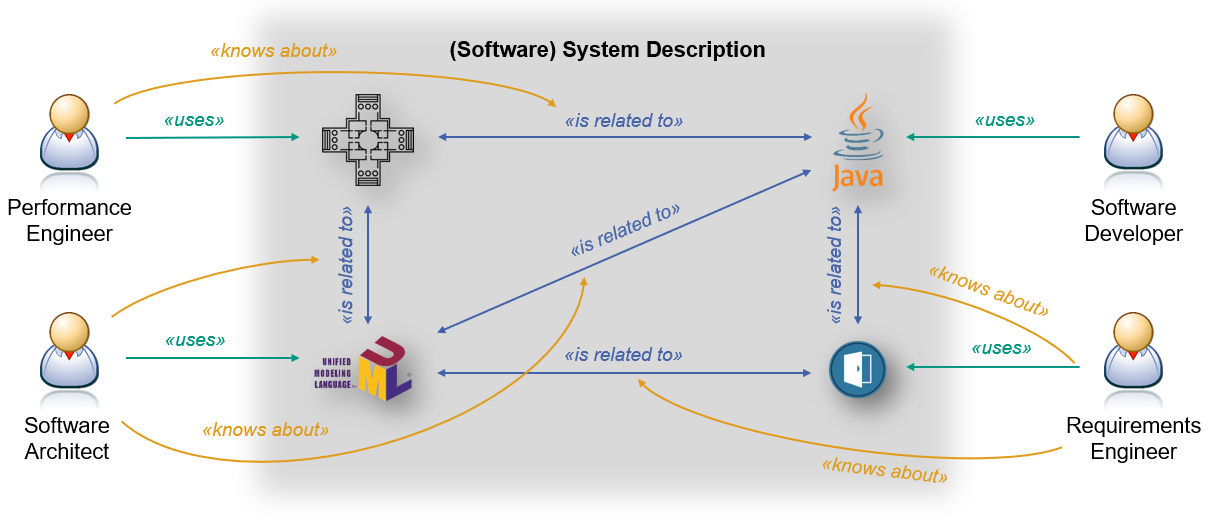
\includegraphics[width=\textwidth]{figures/prologue/introduction/distributed_knowledge.png}
    \caption[Tools and distributed knowledge in engineering processes]{Different tools and roles involved in an exemplary software development process and distributed knowledge about the relations between models of the different tools.}
    \label{fig:introduction:distributed_knowledge}
\end{figure}

\mnote{Distributed knowledge about consistency}
Domain experts deal with the tools and corresponding models they require for their tasks in developing a system.
Usually, each of them is only concerned with a subset of all tools involved in the development of a system.
For example, a performance engineer may be concerned with an instance of the \gls{PCM}, which represents a component-based architecture description of the system, to perform an architecture-based prediction of the system's performance and knows how this description is reflected in the system implementation in Java.
A software architect may use \gls{UML} models for the architecture specification and know how they are related to the implementation as well as to the component-based architecture models in \gls{PCM}.
Finally, a requirements engineer may use IBM Rational Doors and know how they have to be reflected in the architecture specification and implementation to consider the models consistent.
These exemplary relations are depicted in \autoref{fig:introduction:distributed_knowledge}.
No matter whether this is how knowledge is actually present at the different roles in a concrete scenario, it emphasizes that knowledge about the relations between languages and their models will usually be distributed across different experts as soon as multiple models are involved.
In large software systems, a single developer cannot know about all model dependencies~\cite{petrenko2008a}.
In consequence, a process for specifying consistency by means of transformations has to support a kind of \emph{modularity} to foster independent specification of distributed knowledge.
% Maybe discuss that not only binary is case if covered, but also modular multiary case

\mnote{Reuse of consistency specifications}
Furthermore, an automation especially proposes benefits if it is used often.
A specification of consistency and its preservation between common languages, such as \gls{UML} and a programming language like Java, can be reused across multiple projects.
Not each project will, however, use exactly the same tools.
Considering the example in \autoref{fig:introduction:distributed_knowledge}, if the relation between \gls{PCM} and Java was, at least partly, expressed indirectly across the relations between \gls{PCM} and \gls{UML} as well as \gls{UML} and Java, it would not be possible to reuse that specification in another project that only uses \gls{PCM} and Java but omits \gls{UML}.
Thus, parts of the consistency specifications, i.e., specifications for subsets of the tools in a project, should be reusable, comparable to \gls{COTS}.
In consequence, a process for specifying consistency by means of transformations has to support the \emph{independent} specification of \emph{modular} transformations, which can be combined with arbitrary other modular transformations in different contexts.

\mnote{Context assumptions}
To support the context induced by the previous considerations, we focus on combinations of transformations, be they bidirectional or multidirectional, instead of having only a single multidirectional transformation.
We call such a combination a \emph{transformation network}.
To summarize the previous considerations, we need to cover the following context assumptions to the specification of the individual transformations of a network:
\begin{properdescription}
    \item[Modularity:] Transformations are defined in a modular way, i.e., each transformation does only specify consistency and its preservation for a subset of the tools used in an actual development project.
    \item[Independence:] Transformations are defined independently, i.e., each transformation can be developed without considering the contents of the other transformations to be combined with.
\end{properdescription}


\subsection{Orchestration of Transformation Networks}
\label{chap:introduction:consistency:orchestration}

\mnote{Limitations of transformation orchestration}
Combining several modular and independently developed transformations requires their \emph{orchestration}, i.e., the decision in which order the transformations need to be executed to restore consistency.
Existing work proposes, for example, to define an execution order explicitly ~\cite{pilgrim2008a, vanhooff2007UniTI-MODELS} or to derive a kind of topological order~\cite{stevens2020BidirectionalTransformationLarge-SoSym}.
Such approaches either require a manual decision for the orchestration or restrict the execution to specific topologies, such as directed acyclic graphs or trees. %, which limits the kinds of supported transformation networks.
In any case, strong assumptions to the individual transformations or the topology of the supported networks are made.
%To foster distributed development and partial reuse, arbitrary topologies should be supported (Universality, Reusability).

\mnote{Universal combination of specifications}
It is yet unclear how arbitrary modular and independently developed transformations can be combined in a universal way.
%This especially concerns the role of the transformation developer.
It is neither known how a developer can achieve a \emph{correct} transformation network specification, i.e., transformations and an orchestration of them that delivers consistent models when applied, nor how he or she can systematically improve quality attributes of the network such as %\emph{reusability} and 
\emph{comprehensibility}.
%For the role of the transformation user, it is yet unknow how to support him in understanding the reasons whenever transformations fail to deliver consistent models.

%\mnote{Two roles: transformation users and developers}
%Fragmentation addresses challenges of transformations users.
%Challenges of developers yet addressed for binary case.

\begin{figure}
    \centering
    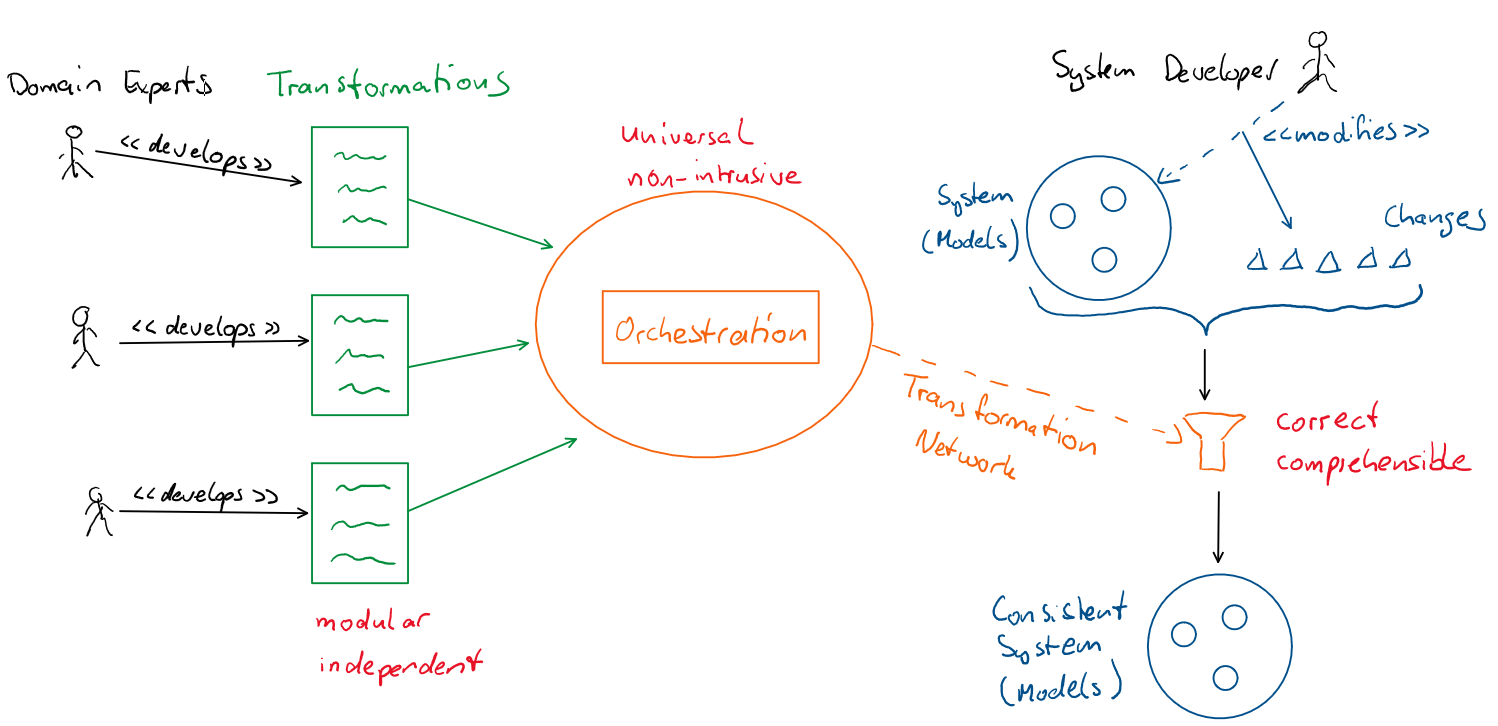
\includegraphics[width=\textwidth]{figures/prologue/introduction/overall_process.png}
    \caption[Process of specifying and executing a transformation network]{The process of specifying and executing a transformation network. 
    % Different domain experts specify transformations, which are combined to a transformation network by an orchestration mechanism that decides which transformations have to be executed in which order. If an actual system is developed and a developer modified models, the network is applied to these models and the performed changes to produce a consistent system description again. 
    Artifacts defined by transformation developers are marked green, artifacts at runtime are marked blue and the artifacts for orchestration and application developed in this thesis are marked orange. The assumed and envisioned properties are denoted in red.}
    \label{fig:introduction:process_overview}
\end{figure}

\mnote{Envisioned properties and process}
Under the assumption of a modular and independent specification of the individual transformation, we aim at an approach for executing transformation networks that has the following properties:
\begin{description}
    \item[Universality:] The approach shall be able to process transformation networks of arbitrary topology. In particular, specific topologies cannot be assumed or prescribed if the assumption of independent development shall be supported.
    \item[Non-intrusiveness:] The approach shall be non-intrusive. When independently developed transformations are combined to a network, they should be treated as black-boxes and there should be no need to adapt them to be used together.
    %It must be possible to combine arbitrary specifications. This means that the approach should not restrict which specifications can be combined, especially not which topology, induced by the specifications (such as only a tree) should be supported. In fact, requirements that all specifications have to fulfill may be defined, but apart from that the usability of one specification should not depend on the existence or non-existence of another.
    \item[Correctness:] The approach shall operate correctly. If it applies transformations to preserve consistency of models, the result must be consistent or indicate an error. The identification and definition of a more precise and appropriate notion of correctness is part of the contributions of this thesis.
    %\item[Reusability:] The approach shall improve reusability. This means that the individual transformations shall be reusable independently.
    \item[Comprehensibility:] The approach shall improve comprehensibility. If the transformations are not able to produce models that are actually consistent, it should support the user in finding the reason for that.
\end{description}
The envisioned process with the involved roles, artifacts and required properties is depicted in \autoref{fig:introduction:process_overview}.
Different domain experts specify transformations, which are combined to a network with an orchestration mechanism that decides in which order transformations have to be executed. If an actual system is developed and a system developer modifies models, the transformations of the network are applied to these models and the performed changes to produce a consistent system description again.

\mnote{Thesis contributions}
In this thesis, we contribute to support the process of building transformation networks that have the defined properties by providing a formal foundation for transformation networks of arbitrary topology and defining a formal notion of correctness for them.
We discuss how correctness of a universal approach to orchestrate and apply the transformations of a network can be achieved by construction or at least by analysis, and which properties the different involved artifacts, such as transformations and their orchestration, have to fulfill for that.
The proposed strategy to orchestrate transformations improves comprehensibility in cases when it is not able to execute transformations such that they deliver consistent models.
Additionally, we classify which kinds of errors can occur when the artifacts are not defined correctly.
We also analyze how topologies of networks affect the desired properties and propose an approach of defining transformations that resolves trade-offs between the envisioned properties.
Finally, we propose an approach to integrate artifacts of arbitrary languages into such a consistency process to ensure that all artifacts describing a system can be kept consistent.

\mnote{Towards detailed problem statement}
In the following, we first discuss the addressed challenges in more detail by considering a specific scenario and generalizing some of the challenges to give a first impression of the issues we have to address.
We then derive two general problem statements from the identified challenges.
Afterwards, we derive our central general research goal and define several questions arising from that, which address the problem statement.
After more precisely specifying the context and assumptions that we make, we give a detailed overview of our contributions.



%%
%% PROBLEM DESCRIPTION -> RESEARCH GAP
%%
\section{Consistency Specification Challenges}

To get an impression of problems arising from the combination of modular transformations, we introduce an exemplary scenario from a software engineering process.
We motivate why we expect that multiple executions of the same transformation can be necessary and discuss some of the issues that can occur in that context.
Afterwards, we generalize that scenario and derive a more precise problem statement.

\mnote{Software engineering scenario}
We consider an extract of a software engineering scenario, in which three roles using three different tools are involved, according to \autoref{fig:introduction:distributed_knowledge}. 
A software developer implements the system with an object-oriented programming language such as Java.
An architect manages the object-oriented architecture of the system with \gls{UML}. 
Finally, a performance engineer uses a component-based representation of the architecture with the \gls{PCM} containing an abstract behavior description at the architecture level to predict the system's performance to evaluate different design options.

\mnote{Contents of \gls{PCM}}
The basic entities in \gls{PCM} models are components, interfaces and data types.
Components are units of reuse that define which interfaces they provide or require and contain abstract service specifications for the operations of the interfaces they provide.
This allows to assemble a system of components by connecting components through their interfaces, such that every required interface of one component is provided by a defined other component.
For the consistency relations between the three languages \gls{PCM}, \gls{UML} and Java, which specify when models of those languages are to be considered consistent, we use the ones proposed by \textcite{langhammer2017a} between \gls{PCM} and object-oriented design, be it \gls{UML} or Java, and the intuitive notion of consistency between \gls{UML} and Java.

\begin{figure}
    \centering
    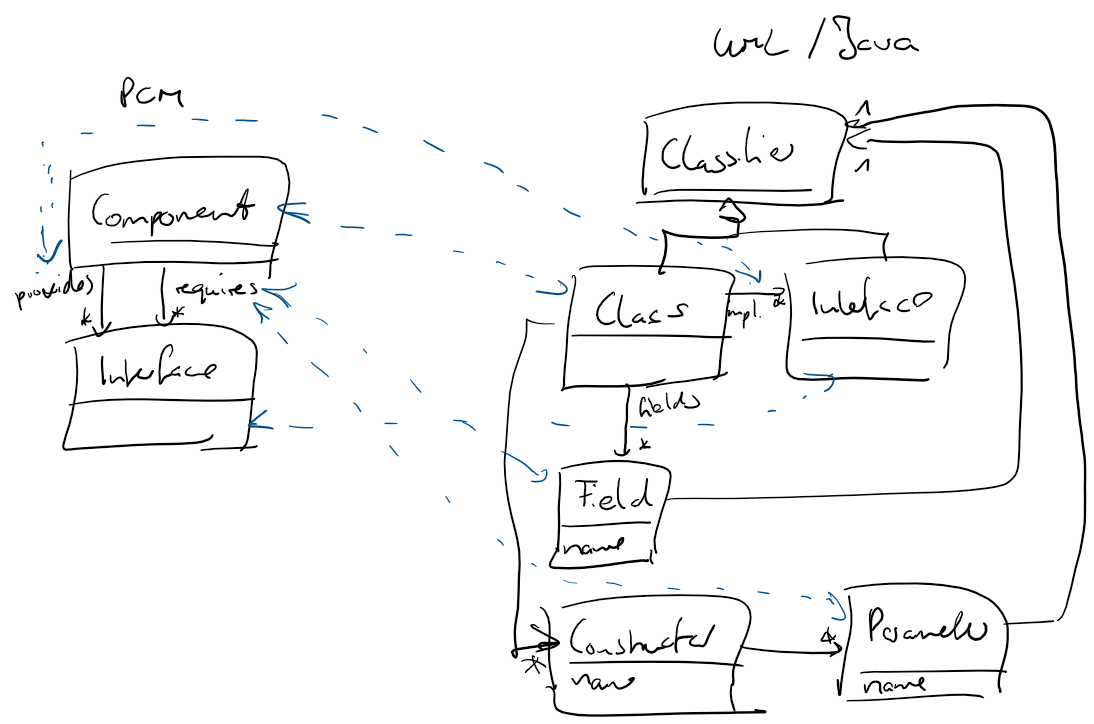
\includegraphics[width=\textwidth]{figures/prologue/introduction/scenario_consistency_relations.png}
    \caption[Consistency relation for PCM and UML/Java]{Extract of consistency relations between component-based architectures in \gls{PCM} and object-oriented design in \gls{UML}/Java according to \cite{langhammer2017a}. Properties are omitted, each element has a least a name.}
    \label{fig:introduction:scenario_consistency_relations}
\end{figure}

\mnote{Consistency relations between \gls{PCM}, \gls{UML} and Java}
Although there are several degrees of freedom to relate \gls{UML} and Java, the extracts that we consider follow a simple one-to-one mapping.
The relevant relations between classes in \gls{PCM} and object-oriented design are depicted in \autoref{fig:introduction:scenario_consistency_relations}.
%We only depict the classes without their properties. Each of them actually has a least a name.
This involves a one-to-one mapping between interfaces and the realization of \gls{PCM} components as classes. 
Provided interfaces in a \gls{PCM} model are realized by interface implementations of the class realizing the component. 
Required interfaces are realized by a field with the type of the interface and constructor parameters that ensure that the required interfaces are set on instantiation of the component.

%% CORRECTNESS
\subsection{Correctness of Transformation Networks}

The central goal of (software) engineering, and thus also the construction of transformation networks as part of the engineering process, is to achieve \emph{correctness} of the developed artifacts.

\subsubsection*{Orchestration Challenge}
\label{chap:introduction:challenges:correctness:orchestration}

% 1. Orchestration problem
\mnote{Single execution of transformations}
When we consider transformations between \gls{PCM} and \gls{UML}, as well as between \gls{UML} and Java, they can transfer each modification to the other models.
For example, adding a \gls{PCM} component creates a class in \gls{UML}, which in turn creates a class in Java.
Although in most cases each transformation only needs to be executed once, there can be situations that require transformation to be executed repeatedly.

\begin{figure}
    \centering
    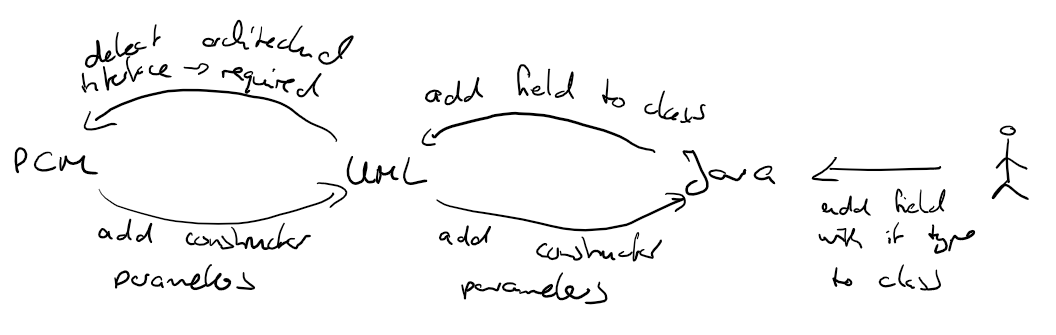
\includegraphics[width=\textwidth]{figures/prologue/introduction/scenario_duplicate_execution.png}
    \caption[Example for transformation orchestration]{Duplicate transformation execution after adding a field representing a required interface to a Java class.}
    \label{fig:introduction:scenario_duplicate_execution}
\end{figure}

\mnote{Multiple executions of same transformation}
In the process depicted in \autoref{fig:introduction:scenario_duplicate_execution}, we assume a system description that contains at least one component and class, respectively, and one interface.
If a developer adds a field to the Java class having the type of the interface, the transformation between \gls{UML} and Java transfers this field to the corresponding \gls{UML} class.
The transformation between \gls{UML} and \gls{PCM} detects that the interface is also represented as an architectural interface in the \gls{PCM} model, thus the field is supposed to represent a required interface in the architectural model.
In consequence, the transformation adds a required interface to the \gls{PCM} component.
Since the consistency relations prescribe each required interface to be represented as a constructor parameter, the transformation also adds a constructor parameter to the class in the \gls{UML} model.
This finally requires the transformation between \gls{UML} and Java to be executed again, because the constructor parameter introduced by the transformation between \gls{PCM} and \gls{UML} must also be added to the Java code.

\mnote{Orchestration challenge}
The example demonstrates that, in general, it is necessary to execute each transformation in a network more than once to achieve a consistent state of the models.
This is always the case if at least two transformations modify the same model, because then the first transformation may need to react the changes of second one again, like in the example the transformation between \gls{UML} and Java needs to react to the one between \gls{PCM} and \gls{UML}, because both modified the \gls{UML} model.
The determination how often and in which order transformations have to be executed is what we call the \emph{orchestration challenge}.

\subsubsection*{Synchronization Challenge}
\label{chap:introduction:challenges:correctness:synchronization}
% 2. Synchronization problem
\mnote{Transformation between \gls{PCM} and Java}
We yet considered that we only have a chain of two transformations, one between \gls{PCM} and \gls{UML} and another between \gls{UML} and Java.
There may, however, also be an overlap of information between \gls{PCM} and Java that cannot be represented in \gls{UML}, which require to also define a transformation between \gls{PCM} and Java.
This is especially the case for behavioral properties, which cannot be expressed in UML class models, such as the functionality defined by Java method implementations and the abstract service specifications in \gls{PCM}.
In consequence, the graph induced by the transformation contains a cycle.

\mnote{Redundancies in transformations}
Instead of only having a transformation for that overlapping information of \gls{PCM} and Java that cannot be expressed across \gls{UML}, the transformation may also contain the relations already expressed across \gls{UML}.
The reasons for that can be independent development and reusability.
Independent development leads to the situation that the developer of the transformation between \gls{PCM} and Java does not know what the transformations to \gls{UML} already express.
Even if the developer has that information, he or she may want to express it again to foster reusability, i.e., to use the transformation between \gls{PCM} and Java in projects in which no \gls{UML} is used or when the transformation is not supposed for a specific network of transformations, comparable to \gls{COTS}.
In consequence, we need to face the situation that multiple transformations propagate the same information, i.e., they contain redundancies.

\begin{figure}
    \centering
    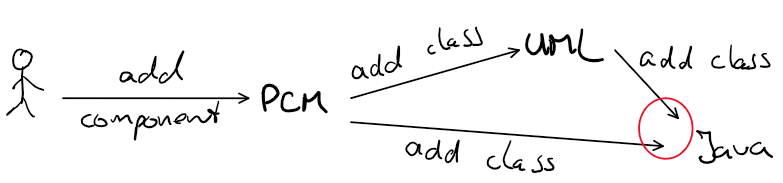
\includegraphics[width=0.8\textwidth]{figures/prologue/introduction/scenario_synchronization.png}
    \caption[Example for transformation synchronization]{Two transformations propagating the same information to Java.}
    \label{fig:introduction:scenario_synchronization}
\end{figure}

\mnote{Two transformation paths creating Java class}
\autoref{fig:introduction:scenario_synchronization} depicts a scenario, in which a user creates a \gls{PCM} component.
The transformations, in consequence, create a \gls{UML} class and, finally, both the transformation between \gls{UML} and Java as well as the one between \gls{PCM} and Java define the creation of an appropriate Java class.
These transformation now have to consider that there may be another transformation that already created that class.
Otherwise, there is the risk of creating a duplicate of that class or of overwriting the already created on.

\mnote{Synchronization challenge}
Such a problem can always occur if two sequences of transformations propagate the same information to the same model. %, like here to Java.
How to achieve that transformations deal with such cases constitutes the \emph{synchronization challenge}.

\subsubsection*{Contradiction Challenge}
% 3. Contradiction problem

\mnote{Equivalence of redundancies}
We have seen that it may be necessary to redundantly define the same consistency relations in different transformations.
This, however, implicitly assumes that they are true redundancies, i.e., that they equally express the relations.
This, in turn, requires all developers to have the same \emph{notion of consistency} between the different tools.

\begin{figure}
    \centering
    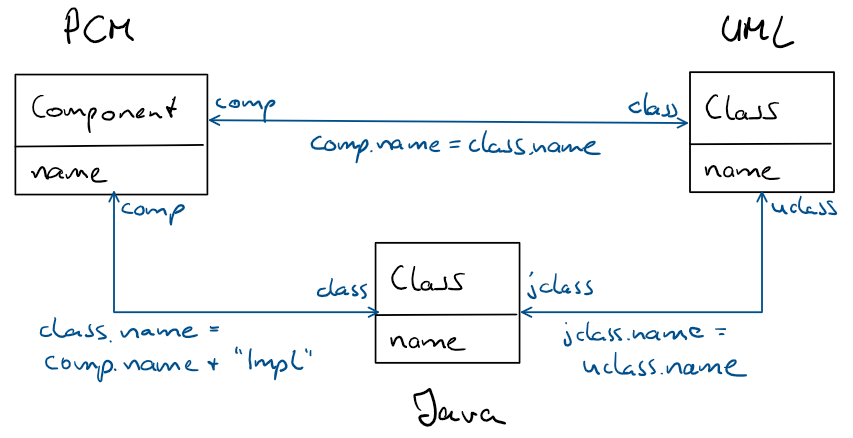
\includegraphics[width=0.8\textwidth]{figures/prologue/introduction/scenario_contradiction.png}
    \caption[Example for transformation contradictions]{Contradicting consistency relations between components in \gls{PCM} and classes in \gls{UML} and Java.}
    \label{fig:introduction:scenario_contradiction}
\end{figure}

\mnote{Contradicting relations}
The example in \autoref{fig:introduction:scenario_contradiction} informally depicts exemplary consistency relations between components and classes.
They are supposed to express that for each a component or class appropriate elements in the other models have to exist with the given name relation.
The constraints for their names can, however, obviously not be fulfilled at the same time.
While the class representations are supposed to have the same name and the \gls{PCM} is also supposed to have the same name as the \gls{UML} class, it is supposed to have the name of the Java class with an \enquote{Impl} suffix, as proposed by \textcite{langhammer2017a}.

\mnote{Different notions of consistency}
Such a situation can occur if the developers of the different transformations have different notions of consistency.
In this case, the performance engineering, who knows about the relation between \gls{PCM} and Java according to the scenario presented in \autoref{fig:introduction:distributed_knowledge}, and the software architect, who knows about the relation between \gls{PCM} and \gls{UML} as well as between \gls{UML} and Java, have different notions about how to represent components in object-oriented design.

\mnote{Non-termination or inconsistent termination}
If the domain experts encode the defined relations in transformations that try to preserve them and execute them after any of the elements is added to a model, the transformations will either terminate in an inconsistent state or never terminate at all.
Executing the transformation for a finite number of times would always result in an inconsistent state, if not removing the element just added by the user.

\mnote{Contradiction challenge}
In consequence, it is important to avoid or detect situations in which transformations with such contradicting constraints in their consistency relations are combined to a network.
We call this the \emph{contradiction challenge}.

\subsubsection*{Problem Statement}

\mnote{Systematic knowledge on correctness challenges}
We have discussed three kinds of issues, which can prohibit that a transformation network terminates consistently, and derived according challenges: orchestration, synchronization and contradiction.
These challenges only exemplify the relevant correctness issues in transformation networks. 
In fact, it is even not systematically known which issues can occur.
Thus, we derive the following general problem statement.

\begin{problemstatement}
    It is unknown how to correctly combine modular and independently developed transformations to networks to yield consistent models after they were changed.
\end{problemstatement}

%% QUALITY PROPERTIES
\subsection{Quality of Transformation Networks}

\mnote{Quality properties of networks}
Like in ordinary (software) engineering, besides the primary goal of producing \emph{correct} artifacts, there are several quality properties that need to be improved.
They can range from properties that are relevant for developers, such as reusability and evolvability, to properties relevant for users, such as performance, scalability and reliability.
This similarly applies to transformation networks as artifacts of the (software) engineering process.

\subsubsection*{Properties and Topology Challenge}

\mnote{Focus on development properties}
In this thesis, we focus on further properties regarding the development of a transformation network, such as reusability and evolvability, rather than properties of its usage, such as scalability.
Reusability is of most importance, because transformation may be used in different contexts within different networks of other transformations.

\begin{figure}
    \centering
    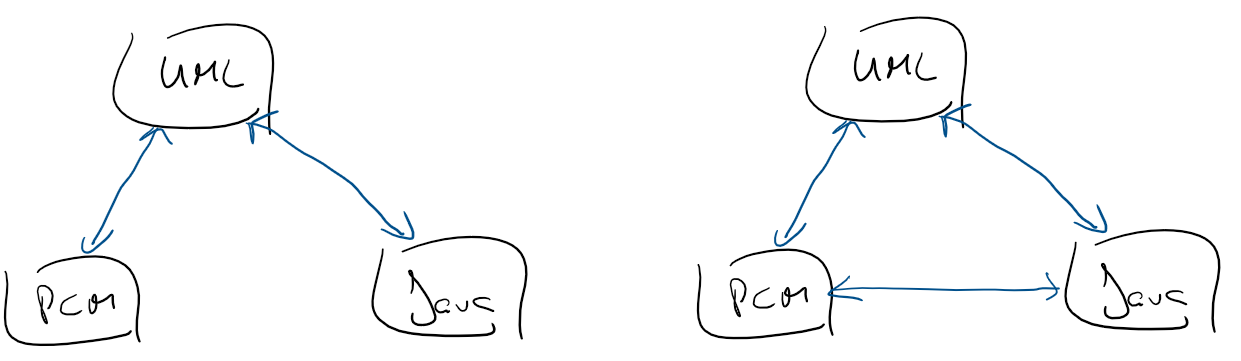
\includegraphics[width=\textwidth]{figures/prologue/introduction/scenario_topologies.png}
    \caption[Example for network topologies]{Different transformation network topologies for \gls{PCM}, \gls{UML} and Java.}
    \label{fig:introduction:scenario_topologies}
\end{figure}

\mnote{Topology extremes}
Consider the two networks depicted in \autoref{fig:introduction:scenario_topologies}.
The networks contain transformation between \gls{PCM} and \gls{UML} as well as between \gls{UML} and Java. 
One of them additionally contains a transformation between \gls{PCM} and Java.
They can be considered as representatives of extremes of transformation networks:
the graph induced by transformations may on the one end be a tree, and on the other be a dense graph.

\mnote{Topologies affect properties}
It is easy to see that properties are directly affected by the network topology.
A dense graph has the benefit of high reusability, because any subset of tools can be used for a development project without loosing consistency.
In the example, the tree network is not applicable in development projects not using \gls{UML}, because then \gls{PCM} and Java cannot be kept consistent.
Additionally, a dense graph profits from universality, because arbitrary relations can be expressed, whereas a tree requires that of three languages there is always one that can express the overlap of the two others.
If there are overlaps between \gls{PCM} and Java that cannot be expressed across \gls{UML}, like discussed for behavioral specifications, a tree cannot be defined.
On the other hand, a tree has the benefit of inherent correctness guarantees.
There are no two paths of transformations between the same two languages.
Thus, no changes can be propagated across two paths to the same model.
This avoid at least two of the three introduced challenges regarding correctness, because neither synchronization problems nor contradictions can occur.

\mnote{Topologies induce trade-offs}
While each kind of topology improves certain properties, it degrades others at the same time.
In other words, topologies induce trade-offs between different properties.
For example, a tree improves correctness, but degrades reusability in comparison to a dense graph.
Deriving how to use this knowledge to mitigate trade-offs and improve different properties at the same time is our \emph{properties and topologies challenge}.

\subsubsection*{Improvement Challenge}

\mnote{Improving properties by specific topologies}
We have seen that topologies directly influence properties of a transformation network.
We will see that with an appropriate strategy of building networks with a specific topology, we can mitigate trade-offs.
Currently, however, there is no known approach and language that supports building transformation networks of specific topologies improving quality properties.
Research approaches did consider approaches and languages for single transformations or for specific composition purposes, such as transformations between the same two languages~\cite{wagelaar2010a,wagelaar2011a}, or chains of transformations~\cite{pilgrim2008a, vanhooff2007UniTI-MODELS}.

\mnote{Improvement challenge}
To relieve the developer from the task of identifying a topology to improve different properties, a universal approach to define an according topology and an appropriate language that supports its definition should be provided.
Investigating such a strategy and design options for an according specification language constitutes our \emph{improvement challenge}.

\begin{integrationcontribution}

\subsubsection*{Integration Challenge}

\mnote{Transformations assume models of specific formalisms}
Finally, we have implicitly assumed that models are developed and thus represented in a format to which transformations can be applied.
Languages for specifying transformations, however, have to assume a well-defined formalism of the languages between they transform~\cite{klare2017models}, thus the models have to follow that formalism.
This is especially problematic for code, which will be relevant for almost every development project.
Although there are tools that wrap code in a specific formalism %, such as JaMoPP~\cite{heidenreich2009a,heidenreich2010a} for using Java code in the Eclipse Modeling Framework, 
recognizing incremental updates of code are still poorly supported.

%\mnote{Models are often implicit}
\mnote{Access to implicit models}
Models are often contained implicitly in code.
This mostly concerns domain models for the software to be developed, but also models to represent code. %of code, such as the Java code representation in the Java Development Tools of the Eclipse Framework~\cite{EclipseJDT}, which has capabilities of recognizing incremental updates.
%\mnote{Lifting artifacts to models}
Lifting such implicit models into a format according to formalisms that allow the application of transformations %and transformation languages 
enables projects using such artifacts to apply transformation techniques to preserve consistency.
For all projects containing such artifacts, this can be seen as a preliminary for applying transformation network, as otherwise only the parts of the projects present in an appropriate formalism can be kept consistent.
In consequence, it can be seen as a \emph{completeness} property of the network.
We denote this as the \emph{integration challenge}.

\end{integrationcontribution}


\subsubsection*{Problem Statement}

\mnote{Impact of topologies and usability for mitigating trade-offs unknown}
We have discussed that topologies affect different correctness and quality properties of transformation network and that they impose trade-offs between them.
It is unclear how that insight can be used to systematically improve different properties by building transformation networks of specific topologies.
Thus, we derive the following problem statement.

\begin{problemstatement}
    It is unknown how to systematically mitigate trade-off decisions between correctness and quality properties, such as reusability and comprehensibility, of transformation networks.
\end{problemstatement}


\subsection{Challenges Overview}

\begin{figure}
    \centering
    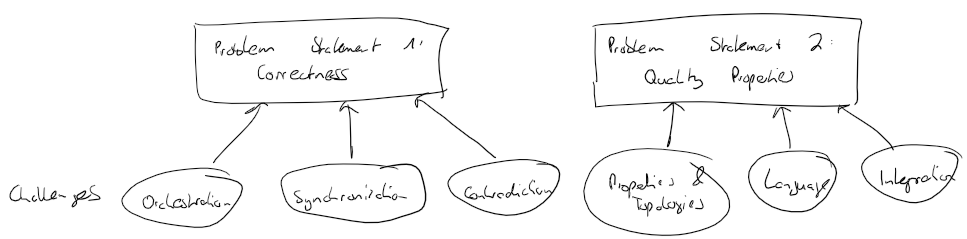
\includegraphics[width=0.9\textwidth]{figures/prologue/introduction/challenges.png}
    \caption[Problem statements and challenges]{The two identified problem statements and their challenges.}
    \label{fig:introduction:challenges}
\end{figure}

\mnote{Summary of problems statements and challenges}
We have discussed several issues regarding the construction of transformation networks.
We summarize the problem statements and challenges in \autoref{fig:introduction:challenges}.
We made two central problem statements, one regarding the correctness of networks and another regarding the improvement of quality properties.
Each of these problems is driven by three challenges.
We identified orchestration, synchronization and contradiction to be central challenges for constructing \emph{correct} transformation networks.
For the improvement of quality properties, we emphasized that the relation between properties and topologies challenges the identification of a topology to mitigate property trade-offs and to define an appropriate strategy and language for that.
\begin{integrationcontribution}
To achieve completeness of a network, we identified the integration challenge. % to integrate all kinds of artifacts into a transformation-based consistency process.
\end{integrationcontribution}


%%
%% RESEARCH OBJECTIVE
%%
\section{Research Objective}

\mnote{Research questions, assumptions and contributions}
We have identified specific challenges that we have to deal with when constructing transformation networks and generalized them into two central problem statements.
In the following, we derive our research goal and the actual research questions that we will answer in this thesis in response to the defined problem statements.
Afterwards, we summarize the context and the assumptions that we make in our work.
Finally, we give an overview of the contributions that we make to answer the defined research questions.

\subsection{Research Goal and Questions}

The central goal of our research can be summarized as follows.
\begin{researchgoal}
Define a notion of correctness for networks of modular, independently developed transformations and classify relevant quality properties.
Provide approaches to systematically improve correctness and quality properties of transformation networks either by construction or by analysis.
\end{researchgoal}

\mnote{Benefits of achieving goal}
The benefits of achieving that goal are twofold.
First, researchers and transformation developers both gain systematic knowledge about how to achieve correctness and improve quality properties in transformation networks.
Second, transformation developers are provided with concrete techniques and languages that help to achieve correctness and improve other properties either by construction or at least by analysis.

\mnote{Parts of research goal}
The research goal consists of two parts, one regarding correctness of transformation networks and one regarding improvement of its quality attributes.
For each of these parts we identify appropriate and fine-grained research questions.

% \subsection*{Properties of Transformation Networks}

% Overall Goal: We want to find out which properties are relevant when building transformation networks and how they are affected by different topologies. This is supposed to help finding ways of systematically improving those properties.

% \begin{researchquestions}{1}
% 	\item \researchquestion{rq:properties}{What are relevant properties and topologies of transformation networks and how do they depend?}
% 	\begin{subresearchquestions}
% 		\item \researchquestion{rq:properties:properties}{Which functional and non-functional properties are relevant when defining transformation networks?}
% 		\item \researchquestion{rq:properties:topologies}{How can network topologies be classified regarding the properties identified in \researchquestionref{rq:properties:properties}?}
% 	\end{subresearchquestions}
% \end{researchquestions}

% \begin{enumerate}[label=\itshape RQ \arabic*.]
% 	% Issue classification
% 	\item Which issues can occur when independently developed \acp{BX} are combined to a network?
% 	\begin{nestedenum}
% 		\item Which failures can occur, when \acp{BX} are combined to a network?
% 		\item What mistakes can be made that lead to failures?
% 		\item How can these mistakes be categorized regarding conceptual levels in the specification process for \acp{BX}?
% 	\end{nestedenum}
% 	\item How are properties of transformation networks affected by the topology?
% 	\begin{nestedenum}
% 		\item Which properties are relevant when defining networks of \acp{BX}?
% 		\item Which topologies of network exist and how do they affect that properties?
% 	\end{nestedenum}
% \end{enumerate}

% \subsubsection*{Evaluation}

% Keine dezidierte Evaluation, lediglich Argumentation


\subsubsection*{Building Correct Transformation Networks} % Correctness of Transformation Networks?

\mnote{Correctness questions}
The first part of our research goal concerns correctness of transformation networks.
We want to know what \emph{correctness} means for transformation networks and which aspects of correctness we can achieve for every network, in particular, which of them we can achieve by proper construction of the single transformations, which we can analyze and for which we need to deal with potential incorrectness until their execution.

\begin{researchquestions}
	\researchquestion{rq:correctness}{When should networks of independently developed transformations be considered \emph{correct} and how can correctness be achieved?}
	\begin{subresearchquestions}
		\subresearchquestion{rq:correctness:notions}{What are relevant notions of correctness in transformation networks and how can they be formalized?}% EV: Argumentation
		\subresearchquestion{rq:correctness:compatibility}{When are the constraints induced by transformations contradictory and how can that be analyzed?}% EV: Proof and empirical application in case study
		\subresearchquestion{rq:correctness:synchronization}{Which requirements must a transformation fulfill for being used in a network in comparison to using it on its own?}% EV: Proof and empirical application in case study
		\subresearchquestion{rq:correctness:orchestration}{How can transformations in a network be orchestrated and which properties can such an orchestration strategy fulfill?}% EV: Argumentation, Examples
		\subresearchquestion{rq:correctness:errors}{Which errors can occur in transformation networks, how can they be classified regarding their avoidability and how severe are they?}% EV: Case Study
	\end{subresearchquestions}
\end{researchquestions}

\mnote{Relation between question and challenges}
\autoref{rq:correctness:notions} is the fundamental question to precisely define what \emph{correctness} means, beyond our yet informally given notion.
\autoref{rq:correctness:compatibility}, \autoref{rq:correctness:synchronization} and \autoref{rq:correctness:orchestration} directly map to the previously identified challenges regarding orchestration, synchronization and contradiction.
Finally, \autoref{rq:correctness:errors} asks for the inverse, i.e., for the case when errors occur due to incorrectness, to find out how incorrectness manifests and how severe it is.


% \begin{enumerate}[label=\itshape RQ \arabic*.]
% 	\setcounter{enumi}{2}
	% % Contradiction analysis
	% \item How can transformations be analyzed regarding contradictions in specified constraints?
	% \begin{nestedenum}
	% 	\item What is an appropriate formalism for describing transformations that can be analyzed regarding potential contradictions?
	% 	\item Which kinds of contradictions can be detected by analyzing transformations following a specific formalism?
	% \end{nestedenum}
	% % Issue avoidance by construction
	% \item How can interoperability of independently developed \acp{BX} be achieved by construction?
	% \begin{nestedenum}
	% 	\item Which kinds of mistakes can be avoided by construction of the individual \acp{BX}?
	% 	\item How can we prove that those mistakes and only those mistakes can be avoided by construction?
	% 	\item How can each of these mistakes be avoided by a transformation developer during independent development of a single \acp{BX}?
	% \end{nestedenum}
	% % Orchestration
	% \item What is an appropriate strategy for orchestrating independently developed \acp{BX} to perform a fixed-point iteration?
	% \begin{nestedenum}
	% 	\item Which strategies for orchestrating a network of \acp{BX} exists and what are their properties?
	% 	\item How should those properties be weighted and which of the strategies should be chosen for orchestration?
	% \end{nestedenum}
% \end{enumerate}

% \subsubsection*{Evaluation}

% \gqm{Functionality}{The analysis can be used to find contradictions in specifications}
% {Does the analysis find contradictions if they exist?}
% {Recall: Ratio of true positives to true positives + false negatives}
% \qm{Does the analysis find contradictions although they do not exist?}
% {Precision: Ratio of true positives to true+false positives}
% \qm{Does the analysis find non-contradictions although they exist?}
% {Ratio of false negatives to false+true negatives}

% \gqm{Functionality}{The techniques to avoid mistakes by construction actually avoid interoperabililty issues}
% {Are the identified failures that can occur complete?}
% {Ratio of number of identified failures to total number of failures}
% \qm{Are the relations of identified mistakes to identified failures correct?}
% {Ratio of failures resolved by fixing the identified mistake to all failures}
% \qm{Does the application of avoidance techniques lead to interoperable transformations?}
% {Ratio of changes that are propagated correctly to those that are not propagated correctly}

% \gqm{Applicability}{The techniques can be applied independently to single transformations}
% {Are there cases in which information about other transformations are necessary to solve issues?}
% {Ratio of number of fixes that require information about other transformation to total number of fixes with user interactions\\
% Ratio of number of fixes that require information about other transformation to total number of fixes without user interactions}


\subsubsection*{Improving Quality Properties of Transformation Networks}

\mnote{Quality properties questions}
The second part of our research goal concerns quality properties of transformation networks.
We want to known how we can systematically improve the quality of transformation networks. 
This includes the identification of properties that are relevant when building transformation networks and how they are affected by different topologies. 
We use this to systematically derive a proper construction approach achieving a specific topology that resolves trade-offs between quality properties. 
%Second, by including models that were not explicitly modelled as such before to allow their integration into a transformation-based consistency process.

\begin{researchquestions}
	\researchquestion{rq:quality}{How can quality properties of transformation networks be improved systematically?}
    \begin{subresearchquestions}
        \subresearchquestion{rq:quality:properties}{What are relevant properties and topologies of transformation networks?} % EV: Argumentation
		\subresearchquestion{rq:quality:topology}{How can topologies of transformation networks improve quality properties of transformation networks?} % EV: Argumentation
		\subresearchquestion{rq:quality:language}{How can a specialized language support the specification of a network topology that improves quality properties?} % EV: Proof-of-concept and case study
        \begin{integrationcontribution}
            \subresearchquestion{rq:quality:process}{How can software development artifacts be integrated into a transformation-based consistency process?} % EV: Case study
        \end{integrationcontribution}
	\end{subresearchquestions}
\end{researchquestions}

\mnote{Relation between question and challenges}
\autoref{rq:quality:properties} and \autoref{rq:quality:topology} directly map to the properties and topologies challenge for identifying how topologies affect properties and how to use them for improving quality properties.
\autoref{rq:quality:language} then maps to the language challenge for designing an appropriate language that supports the construction of an appropriate topology.
\begin{integrationcontribution}
    Finally, \autoref{rq:quality:process} maps to the integration challenge for lifting artifacts to models that can be used in a transformation-based consistency process.
\end{integrationcontribution}

% \begin{enumerate}[label=\itshape RQ \arabic*.]
% 	\setcounter{enumi}{5}
% 	\item How can a topology of transformation be build that optimizes non-functional properties of transformation networks?
% 	\begin{nestedenum}
% 	    \item How can transformation contradictions be avoided by language design? %uniqueness of consistency specification and consistency among themselves achieved by language design?
% 	    \item How can modularity be achieved in a way such that an arbitrary set of metamodels for which consistency is specified can be used in an actual project?
% 	\end{nestedenum}
% 	% Building tree topologies
% 	\item How should a language specific for multi-model consistency be defined that supports a non-functional property-optimizing topology definition?
% 	\begin{nestedenum}
% 		\item What are the design decisions for such a language?
% 	\end{nestedenum}
% \end{enumerate}

% \subsubsection*{Evaluation}

% \gqm{Functionality}{Concept and language can achieve consistency between several models}{How many model changes in a case study can be properly kept consistent?}{Ratio of successfull test cases}

% \gqm{Practicality}{The assumption of defining a tree of \commonalities is achievable in practice}{Is the definition of cross-tree relations necessary in a case study?}{Number of cross-tree relations in a case study compared to number of relations}

% \gqm{Practicality/Benefit}{A specific language improves conciseness of consistency specifications}{How much more concise is the specification for a case study compared to a definition with direct transformations?}{Number of SLOC with \commonalities compared to number of SLOC with \reactions for same case study}

% Diskussion: Erreichen der Modularität auch evaluieren? Ist per Konstruktion gegeben, könnte man aber natürlich auch noch auswerten (bringt aber nichts).



%% CONTEXT AND ASSUMPTION
\subsection{Context and Assumptions}
\label{chap:introduction:objective:assumptions}

\mnote{Model-driven processes}
In this thesis, we consider the context of model-driven development processes, be it software or software-intensive technical systems.
Thus, we assume that the system under construction is described by several models containing information about different extracts or properties of the systems.
We assume that they usually share some overlap of information.
Our discussions will focus on software development artifacts.
As long as they follow the same formalisms, however, the insights and techniques may be applied to artifacts from arbitrary domain.

\mnote{Distributed knowledge and independent development}
We assume that the knowledge about different transformations to be combined to a network is distributed.
To foster the development of transformations that can be used as \gls{COTS}, we assume that transformations are developed independently.
Thus, transformations may not be adapted to be used within transformation networks.

\mnote{Consistency relation types}
We do not restrict the kinds of relations between models to keep consistent  in any way.
We will, however, discuss different types of consistency and their relations to different kinds of processes to preserve consistency in \autoref{chap:networks:notions:types}.
In fact, our contributions, although theoretically not restricted to that, will be best applicable to a kind of \emph{structural} dependencies rather than \emph{behavioral} dependencies.

\mnote{Semi-automatism}
Finally, transformations may not always be able to restore consistency on their own, because necessary information to do so is missing.
For example, a developer may introduce a class in Java and a transformation has to decide whether that class shall represent a component in \gls{PCM} or not.
That problem can either be solved by requiring the class to fulfill certain patterns, like containing \enquote{Component} in the class name, or by asking the user about his intent.
In cases where information is transformed to a semantically richer model, often further information about how to transform is necessary.
\textcite[p. 57]{kramer2017a} provides a classification for different levels of automation, starting from no automation over suggestions and semi-automated repair to fully automated repair.
In this thesis, we assume that consistency is preserved in a fully automated way, thus excluding the semi-automatic case.
We will finally discuss how our finding generalize to the case where user decisions need to be included.

% Focus on development, rather than usage -> motivate comprehensibility with developer, not with user


%% CONTRIBUTIONS
\subsection{Contributions}

\begin{figure}
    \centering
    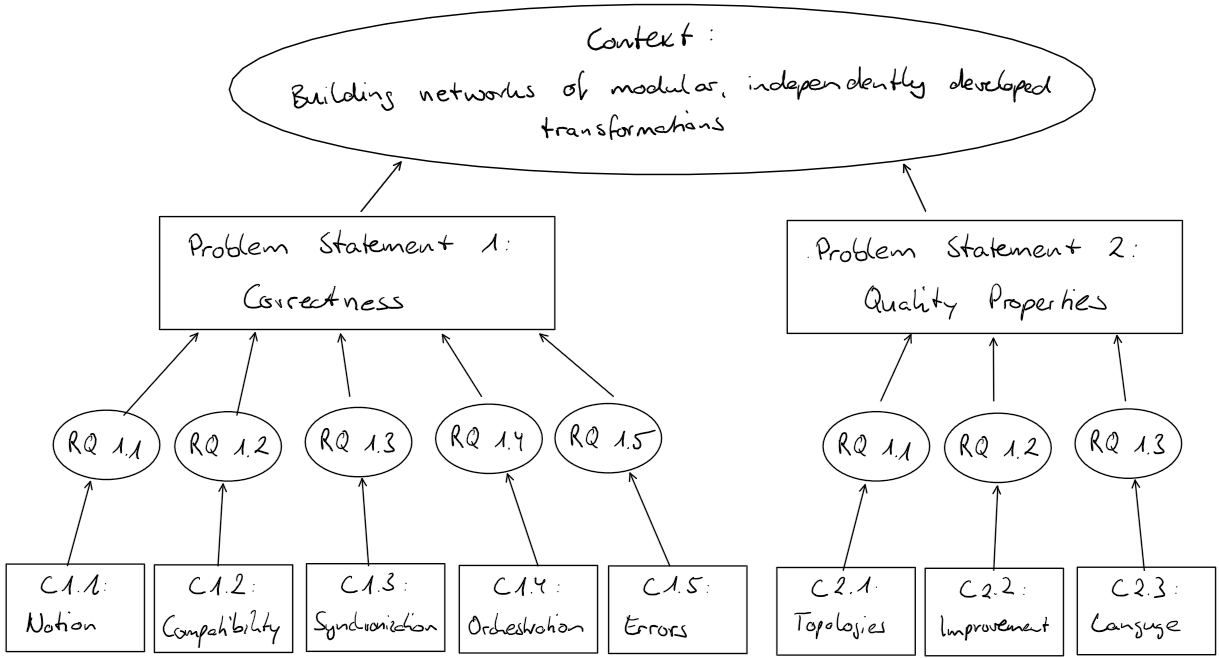
\includegraphics[width=\textwidth]{figures/prologue/introduction/context_problem_eq_contribution_relations.png}
    \caption[Context, problems, research questions and contributions]{Relation between context, problem statements, research questions and contributions}
    \label{fig:introduction:context_problem_rq_contribution_relations}
\end{figure}

\mnote{Contribution structure}
The contributions that we make in this thesis are structured along the same dimensions as the problems and the research questions, namely correctness and quality properties.
The contributions directly map to the research questions.
\autoref{fig:introduction:context_problem_rq_contribution_relations} gives an overview of the relations between the context of our work, the problem statements, the research questions and the contributions that we make.

We make the following contributions regarding transformation network correctness.
\begin{contributions}
    \contribution{contrib:correctness:notion}{Notion}{We discuss different notions of correctness for transformation networks and precisely define the one relevant for our context. We derive that compatibility, synchronization and orchestration constitute the relevant correctness notions.}
    \contribution{contrib:correctness:compatibility}{Compatibility}{We precisely define a notion of compatibility to express when transformations contain contradictory constraints. We propose an approach that validates compatibility of transformations and prove its correctness.}
    \contribution{contrib:correctness:synchronization}{Synchronization}{We discuss how synchronization can be achieved for transformations defined with existing transformation languages. We prove that transformations fulfilling a specific property can be applied in transformation networks. %We make a case distinction over all possible synchronization cases to derive a complete list of problematic synchronization cases. 
    We provide an algorithm to execute the transformation in that case and propose a strategy to fulfill the required property by construction.}
    \contribution{contrib:correctness:orchestration}{Orchestration}{We prove that transformations, in general, can neither be executed only once nor an arbitrary number of times in a fixed-point iteration without the risk of non-termination. We prove that finding an execution order of the transformations that yields consistent models is an undecidable problem and discuss why we cannot make restrictions to the transformations to achieve its decidability. We propose an algorithm for orchestration that executes the transformations according to a well-defined strategy and helps to find the cause in cases it does not return consistent models.}
    \contribution{contrib:correctness:errors}{Errors}{We systematically derive which errors can occur when correctness of a transformation network is not given. We also empirically evaluate the probability of the different errors to occur to classify their severity and thus the importance of avoiding them.}
\end{contributions}

We make the following contributions regarding the improvement of quality properties of transformation networks.
\begin{contributions}
    \contribution{contrib:quality:topologies}{Topologies}{We discuss how different quality properties of transformation networks are affected by the network topology. We derive that trade-off decisions have to be made between the improvement of different properties.}
    \contribution{contrib:quality:improvement}{Improvement}{We propose a strategy for building a specific network topology based on auxiliary models, which make the consistency relations explicit in terms of models rather than transformations. We show that this approach systematically improves different quality properties and mitigates necessary trade-off decisions.}
    \contribution{contrib:quality:language}{Language}{We propose a specialized language for the definition of a network according to the strategy of \autoref{contrib:quality:improvement}. 
    We discuss different design options for the language and its operationalization.}
    \begin{integrationcontribution}
        \contribution{contrib:quality:integration}{Integration}{We propose an approach for lifting existing models, which are only implicitly encoded in code, to an explicit representation according to a modeling formalism. It enables the usage of implicit models in a model-driven development process.}
    \end{integrationcontribution}
\end{contributions}


\subsection{Expected Benefits}

\mnote{Overall benefits}
The contributions that we make in this thesis provide several benefits for researchers, developers of transformations and transformation networks, as well as transformation (network) users.
All of them profit from systematic knowledge about what \emph{correctness} means for transformation networks, how correctness is affected and can be guaranteed, and about relevant \emph{quality properties} in transformation networks as well as how they can be improved.
The contributions, however, have an intended focus on supporting transformation and transformation network developers. 

\mnote{Benefits for researchers}
Researchers can base on our definitions for correctness of transformation networks and can thus precisely contribute to particular parts of the defined correctness notions, e.g., by approaches to achieve correctness, with explicitly knowing how and which kinds of potential errors of transformation networks are affected by that.
Additionally, they can base further research on the insights about trade-offs between quality properties induced by different network topologies.

\mnote{Benefits for transformation (network) developers}
The developers of actual transformation networks can be separated into the developers of the individual transformations and the ones combining them to a network.
The development of individual transformations is supported by the provision of systematic approaches to build transformations that can be used within networks, especially in terms of supporting synchronization.
Transformation network developers benefit from the knowledge that they have to deal with undecidability of orchestration, i.e., of finding an execution order for transformations.
They also benefit from approaches to validate transformations they want to combine regarding compatibility, an actual and practical orchestration strategy to execute transformations, and an approach to build networks that mitigate trade-offs between quality properties.

\mnote{Benefits for transformation (network) users}
Finally, the users of a transformation network, i.e., the ones who develop a system using a transformation network to preserve consistency of its artifacts, benefit from the ability to use networks, for which correctness was systematically achieved, at all.
They also profit from an orchestration strategy that supports them in finding and understanding the reasons why the networks may not be able to process certain changes to preserve consistency.



%%
%% OUTLINE
%%
\section{Thesis Outline}

\todo{Write outline}

First some general considerations, notation, formal basis etc.

Structured along correctness / quality properties.
Each chapter maps to one of the defined contributions

Reading process: Correctness and quality properties are almost independent, so possible to start with any of the parts. Within the parts, consecutive reading recommended.
However:
Correctness: Start with notion and compatibility chapter, then proceed with any of the following, no strict dependencies. Errors hard to understand without rest.
Quality (read first chapter of correctness first): First three chapters depend on each, so do not jump. 
\begin{integrationcontribution}
    Fourth chapter (integration) is independent.
\end{integrationcontribution}

In each chapter, we recapture the research question we want to answer in the beginning and point out the contribution that we make with that chapter and we close the chapter with the central insights that the chapter gave.


%%
%% OLD: COPIED FROM PAPERS
%%

%\begin{copiedFrom}{DocSym}

%\section{From DocSym}
%\todo{Clearly introduce running example, removed from content section!}
%\todo{Introduce set notation, say that is it not practically applicable and a strong simplification, but just used to illustrate the problems and solution approaches} % Done at the end
%\todo{Introduce transitive operator R1 o R2 = (R1 u R2) * $\backslash$ (R1 u R2)} % Done at the end

%\todoConference{The problem the research intends to solve, the target audience of this research, and a motivation of why the problem is important and needs to be solved.}

%\acl{MDSD} proposes the usage of models as primary artifacts of the %software 
%development process~\cite{stahl2006a}. 
%Those models describe different system properties for the interests of specific stakeholders, known as \emph{multi-view modelling}, or at different abstraction levels, representing refinements. In both cases, the models describe the same system and are thus not disjoint but contain redundant or dependent information. 
%\todoErik{Wieder: Die beschreiben ja keine Abstraktion, die sind eine Abstraktion. \enquote{Domains of the system} klingt auch komisch, ich weiß zwar, was Du meinst, aber nenne es nicht \enquote{domain}, sondern lieber \enquote{properties}}
%Developers must be aware of those dependencies to ensure that models are modified consistently. 
%Otherwise, the deployed software, which is derived from those models, will potentially not operate correctly.
%\todoErik{Lenkt den Fokus etwas zu stark auf Korrektheit, die wir nicht formal beweisen. Es geht ja nicht nur darum, daß die Software nicht korrekt arbeitet -- möglicherweise tut sie das ja, obwohl die Modelle inkonsistent sind, und das Problem tritt erst bei der Wartung/Evolution auf.}

%In large software systems, a single developer cannot know about all dependencies~\cite{petrenko2008a}, %which can be formulated as \emph{consistency constraints} and 
%in the following referred to as \emph{consistency relations}, which inevitably leads to inconsistencies. 
%Therefore, automated mechanisms that preserve consistency according to those consistency relations are necessary. 
%For that purpose, incremental, bidirectional model transformations %or specialized model synchronization approaches 
%are commonly used. However, most research considers \emph{binary transformations}, restricted to pairs of models, and does not explicitly consider consistency between more than two models~\cite{stevens2017a}, which we refer to as \emph{multi-model consistency}.
%In general, keeping more than two models consistent is currently not researched well.
%Model transformations can either be specified imperatively or declaratively. They differ in who operationalizes the preservation of constraints that have to hold, in the first case the transformation developer and in the second case an automated mechanism of the transformation language. This is why we do not explicitly distinguish these approaches, as all problems apply to both approaches and only different roles have to deal with them. 
% Model transformations can either be specified imperatively, such that the transformation developer has to define how to react to a change, or declaratively, such that the transformation developers only the constraints that have to hold and an automated mechanism derives an imperative operationalization from that.
% We will not explicitly distinguish these approaches, as the identified problems and our solution proposals apply to both. The only difference is that in imperative approaches the transformation developer has to deal with them and in declarative approaches the developer of the transformation language has to consider them when defining the generation of the operationalization.

% Although it is possible to combine binary transformations by transitively executing them, it is yet unclear what problems may arise from that, especially if each transformation is developed independently and treated as a black box.
% We will exemplify this on the simple example in \autoref{fig:prologue:binary_combination_example}, in which consistency relations define a mapping of a component in an \ac{ADL} to a class in object-oriented design, which is again represented by an implemented class in Java code. 
% The name of the class is defined to be the component name with an \enquote{Impl} suffix (cf.~\cite{langhammer2017a}).
% When all these relations are expressed in transformations, it is, for example, possible that both transformations from \ac{ADL} to Java, once over \ac{UML} (\ref{fig:prologue:binary_combination_example:R1} and \ref{fig:prologue:binary_combination_example:R2}) and once directly (\ref{fig:prologue:binary_combination_example:R3}), create a Java class after creating an \ac{ADL} component.
% We refer to that as an \emph{interoperability problem}.
% The transformation specification %or its execution engine 
% would have to avoid an overwrite and therefore have to consider dependencies between transformations, using, for example, a shared trace model.
% In general, an interoperability problem is an unexpected behavior of transformations, which only occurs if they are executed transitively, but not if each is executed on its own. %, although all preserve the same consistency relations.

% Additionally, it is easy to see that %specifying multi-model consistency with combinations of 
% combining binary transformations leads to trade-off decisions.
% The ternary relation %between the three metamodels 
% can either be expressed by three binary transformations between all pairs of metamodels or by two binary transformations with the third being %expressed by the transitive 
% the combination of the two others.
% The first option leads to redundancies in the specifications, as each pair of transformations has to have an equal semantics than the third.
% For example, the \ac{ADL} to Java transformation for \ref{fig:prologue:binary_combination_example:R3} must be equal to the combination of the transformations \ac{ADL} to \ac{UML}~(\ref{fig:prologue:binary_combination_example:R1}) and \ac{UML} to Java~(\ref{fig:prologue:binary_combination_example:R2}).
% Consequently, those transformations may be incompatible if not correctly defined, e.g., by leaving out the suffix addition in the transformation for \ref{fig:prologue:binary_combination_example:R3}.
% %As an alternative, the second option is express the ternary relation with two binary consistency relation specifications.
% %For example, specification \ref{fig:example:R3} can be interpreted as a combination of \ref{fig:example:R1} and \ref{fig:example:R2}.
% An alternative is to omit the transformation for \ref{fig:prologue:binary_combination_example:R3} by transitively executing the two others.
% However, in this case, modularity is reduced, because it is not possible to use only Java and the \ac{ADL} to develop a specific system and omit the \ac{UML}.
% %Additionally, comprehensibility decreases, because the relation between \ac{ADL} and Java is only expressed transitively. 
% %This becomes more problematic if transformation paths have a length higher than two.
% We refer to this as \emph{specification trade-offs}.

% \begin{figure}
%     \centering
%     \begin{tikzpicture}

    \node[uml class, align=center, minimum width=10em] (component) {\umlcomponentlabel\\[-0.3em] \small PaymentSystem};
    \node[above=0em of component.north, anchor=south] (adl_label) {\textit{ADL}};
    
    \node[uml class, minimum width=10em, below left=2.15em and 7.5em of component.south, anchor=north, font=\small] (uml_class) {PaymentSystemImpl};
    \node[above right=0em and 1em of uml_class.north west, anchor=south west] (uml_label) {\textit{UML}};
    
    \node[draw, minimum width=10em, below right=2.15em and 7.5em of component.south, align=left, anchor=north, font=\small] (java_class) {
    \textbf{class} PaymentSystemImpl \{ \\[-0.3em]
        \hspace{1em} {\tiny // \ldots} \\[-0.3em]
    \}
    };
    \node[above left=0em and 1em of java_class.north east, anchor=south east] (java_label) {\textit{Java}};
    
    \draw[latex-latex, dashed, thick=false] (component) -- node[above left=-0.5em and 0.5em] {\mylabel{fig:prologue:binary_combination_example:R1}{$R_1$}} (uml_class);
    \draw[latex-latex, dashed, thick=false] ([yshift=-1.5em]uml_class.north east) -- node[above] {\mylabel{fig:prologue:binary_combination_example:R2}{$R_2$}} ([yshift=-1.5em]java_class.north west);
    \draw[latex-latex, dashed, thick=false] (component) -- node[above right=-0.5em and 0.5em] {\mylabel{fig:prologue:binary_combination_example:R3}{$R_3$}} (java_class);
    
\end{tikzpicture}
%     \caption{Example models with binary consistency relations}
%     \label{fig:prologue:binary_combination_example}
% \end{figure}

%Although specific approaches for expressing multiary relations, rather than using combinations of binary relations, could be developed, there are some reasons for adhering to binary transformations.
%Instead of developing approaches to express multiary consistency relations, there are reasons to adhere to binary transformations, and to research their combinability.
%As stated by \textcite{stevens2017a}, %there are especially strong practical reasons, as 
%it is hard enough to think about binary relations. %between pairs of models.
%Defining multiary relations would require a knowledge about the relations between all metamodels used to describe a system.
%Additionally, each domain expert, who specifies transformations, %in practice, 
%will usually only have knowledge about the relations between two or at most a rather limited set of metamodels. %, but not of all involved metamodels. %, which would be necessary to define multiary relations.
%Thus, it is a natural goal to make the modular specification of consistency based on binary transformations possible.
%In the proposed thesis, 
%We therefore plan to make the following contributions to research on multi-model consistency preservation:
%\todoErik{Ich fänd's cool, wenn die Probleme auch irgendwie hervorgehoben sind, und Du die Beiträge schon auf die Probleme beziehen kannst, also Mini-PIBA für jedes Deiner identifizierten Probleme. Würde aber erst die Probleme formulieren, dann den IBA-Teil so wie unten (wobei bei manchen noch die Beschreibung des Benefits fehlt).}
% \begin{description}[leftmargin=\parindent]
%     \item[Transformation interoperability.] %Under the assumption that 
%         When several binary transformations are developed independently, they must be combinable in a black box manner, introduced as the \emph{interoperability problem}. We will therefore identify problems that can arise from that combination %of transformations 
%         and develop a catalog of patters that can be followed by the transformation developer or language to achieve \emph{non-intrusive} interoperability of binary transformations.
%     \item[Decomposition of consistency relations.] 
%         The usage of binary transformations for multi-model consistency preservation leads to \emph{specification trade-offs} regarding essential challenges. We will provide a classification of those challenges and investigate the influence of the way in which transformations are specified on them.
%         %Decomposing the underlying consistency relations into independent sub-relations allows a partial optimization regarding those challenges.
%         %We will therefore investigate how consistency relations can be decomposed into independent subsets.
%         We will especially investigate how consistency relations can be decomposed into independent subsets, as this allows a partial optimization regarding those challenges.
%     %We will identify relevant properties of consistency specifications, which have to be considered when defining those specifications as they introduce trade-off decision. We already motivated some of those properties above and give a more detailed overview in \autoref{sec:multimodelconsistency}.
%     \item[Make common concepts explicit.] 
%         Metamodels often represent the same concepts in different ways. As another contribution to reduce \emph{specification trade-offs}, we propose an approach to make these common concepts explicit to improve comprehensibility of transformations and to improve their modular reuse.
% \end{description}

% We propose an approach for multi-model consistency based on \aclp{VOMM}. 
% In those virtual metamodels, dependencies between metamodels, which we refer to as \emph{consistency relations}, are made explicit by representing common concepts, whereas in model transformations, which we refer to as \emph{consistency preservation specifications}, they are specified implicitly. 
% The envisioned benefit is an inversion of the above mentioned properties. 

%Throughout this paper, we use a simplified notation for metamodels and heir consistency relations to ease their illustration. 
%We consider metamodels to be sets of elements and consistency relations to be sets of symmetric, binary relations between those elements.
%To ease the representation of combinations of consistency relations, we define the concatenation operation for two consistency relations $R_1$ and $R_2$ as:
%\begin{equation*}
%    R_1 \concat R_2 \coloneqq \{(x,y)\, |\, \exists t: x\, R_1\, t\, R_2\, y \}.
%\end{equation*}
%This is the subset of the transitive closure of two relations that contains only the relations transitively defined over $R_1$ and $R_2$.
%It can be also expressed as the natural join of $R_1$ and $R_2$ with an additional projection that removes the common elements of both relations.
%The operator is commutative since the relations are assumed symmetric.

% \todoErik{Würd ich bei so einem kurzen Paper weglassen. (Ich würde es auch oft bei langen Papern weglassen. :-))}
% In this paper, we first discuss related work in \autoref{sec:relatedwork}. 
% In \autoref{sec:approach}, we give an overview of our planned contributions by explaining the problems in detail and sketching our solution approaches. %we first discuss interoperability problems arising from the combination of independently developed binary transformations and give an overview on envisioned solution patterns.
% %We then give an introduction to the yet identified challenges inducing trade-off decisions during transformation development.
% %From this, we derive the consideration of consistency relation composition and an approach to make common concepts explicit.
% % We then discuss problems arising from the black-box combination of binary transformations and give an overview on envisioned solution patterns.
% % In \autoref{sec:vomms}, we introduce our approach to make overlaps of metamodels explicit to improve properties of multiary consistency specifications.
% Finally, we discuss the current state and planned evaluation in \autoref{sec:status} and conclude the paper in \autoref{sec:conclusion}.


% \begin{itemize}
%     \item Motivation MDSD
%     \item Several models describe single system
%     \item Information overlap between models, e.g. component architecture and code, ref to Michael
%     \item Developers must be aware of redundancies and dependencies, otherwise inconsistencies
%     \item Best: Make redundancies/dependencies explicit for (semi-)automated mechanisms for preserving consistency
%     \item Incremental model transformations can be used (refs) or specialized model consistency or model synchronization approaches (refs)
%     \item Existing approaches only concern consistency preservation between instances of two metamodels
%     \item If more than two models are involved, these approach would require that consistency preservation is executed transitively
%     \item From that, problems arise
%     \begin{itemize}
%         \item Inconsistent consistency specifications: Consistency specifications between different metamodels must be consistent. E.g. having 3 metamodels, a consistency specification between two of them can be contradictory to the two other
%         \item Consequence: Result of a modification depends on the order in which consistency specification are evaluated or even results in propagation cycle due to alternating changes -- EXAMPLE
%         \item Ordering problem: Preserving consistency after a change can require several changes in other models. The order in which they are executed can produce different results -- EXAMPLE
%         \item Confluence problem: Changes can be propagated across several paths, if more than two models are involved. This can result in conflicts, if the propagation confluences in one model. E.g. it can be necessary to create a metaclass instance in that model to preserve consistency. All confluencing change propagations require the creation of an element, but how can you achieve that only the first one creates it and the other see the new element and reference it instead?
%     \end{itemize}
% \end{itemize}

%\todoHeiko{Define metamodel vs. \modelinglanguage, Use \modelinglanguage or DSL?}
%\todoHeiko{Say: code is also a model}
%\todoHeiko{Define: \emph{consistency relation} for existing relationships between metamodels that require consistency preservation and \emph{consistency preservation specification} for mechanisms that semi-automatically preserve consistency according to an existing consistency relation}
%\todoHeiko{We refer to the process of preserving consistency due to defined consistency preservation specifications as \emph{change propagation}, as a performed change resulting in the violation of consistency relations leads is propagated to restore consistency -- Besser change propagation überall weglassen.}
%\todoHeiko{Introduce trace links and their necessity for identifying corresponding elements according to consistency relations (prescriptive vs. descriptive)}


%\todo{Klarmachen, dass es immer darum geht Konsistenzrelationen durch bidirektionale, binäre Transformationen auszudrücken. Das ist die Baseline.}

%\todo{Klarmachen, dass Kombination binärer Transformationen der state-of-the-art ist.}

%\end{copiedFrom} % DocSym


% \begin{copiedFrom}{SoSym MPM4CPS}

% \section{From SoSym MPM4CPS}

%%
%% Scope: Building large systems of many models
%%
%The scale of modern software systems and their embedding into cyber-physical systems leads to a high and even increasing complexity of systems to be built. 
%To handle that complexity, different roles operate on appropriate extracts and abstractions of the system under construction described by different models or views.
%Such a fragmentation of information across different models is common at a high level, i.e., mechanical, electrical and software engineers usually use different models and associated tools to describe a system in their domain.
%Additionally, different models can be used on a low level by engineers from the same domain, such as software engineers using different models for architecture specification, behavior development and deployment.
%For example, the development of \acp{ECU} software in automotives comprises different tools or standards for specifying the system and software architecture, such as SysML~\cite{sysml} or AUTOSAR~\cite{scheid2015autosar}, for defining the behavior, such as MATLAB/Simulink~\cite{simulink} or ASCET~\cite{ascet}, and for defining the deployment on multi-core hardware architectures, such as Amalthea~\cite{amalthea, wolff2014a}.
%Since all these models describe the same system, they usually share an overlap of information in terms of dependencies or redundancies, which can lead to inconsistencies if overlapping information is not modified properly in all models.
%Recent research investigated such dependencies between ASCET and SysML~\cite{giese2010a}, as well as Amalthea and how to resolve them~\cite{mazkatli2017ase,mazkatli2016ma}.

%%
%% General solution: incremental BX combined to a network
%%
%For resolving inconsistencies, different approaches have been developed.
%Incremental model transformations are a common approach to resolve such inconsistencies by enabling developers to explicitly specify how inconsistencies can be resolved (semi-)automatically. 
%Especially bidirectional model transformations~\cite{stevens2010sosym}, which specify the relations between two metamodels and routines how consistency of their instances can be restored, are well suited and well researched.
%Relating more than two metamodels can either be achieved by defining a multi-directional transformation between all of them or by specifying bidirectional transformations %transformations between pairs of metamodels, i.e., bidirectional transformations, 
%between pairs of them in a modular way and combine them to a network that is able to check and preserve consistency between several models.
%In consequence, a more reasonable option is to specify transformations between pairs of metamodels, i.e., bidirectional transformations, in a modular way and combine them to a network that is able to check and preserve consistency between several models.
%\begin{example}
% \autoref{fig:prologue:three_persons_example} exemplifies these different possibilities at the example of relation of transformations between three simple metamodels for persons, employees and residents.
% We use an informal notion of consistency, defined more precisely later on, which requires that if any person, employee or resident is contained in a model, there must also be the other two elements with the same names, addresses, incomes and social security numbers. %fulfilling a specific relation of their properties.
% %That relation includes that names, addresses, incomes and the social security numbers % (\texttt{socsecnumber}) 
% are equal.
% This relation can either be expressed as a ternary relation, denoted as $R_{PER}$, or as three binary relations $R_{PE}, R_{PR}, R_{ER}$.
% In such a simple scenario a single developer may be able to define all these relations.
% However, in a more complex scenarios, like the relations between the previously mentioned SysML, Amalthea and ASCET metamodels, there may not be a single person having the knowledge about all these dependencies~\cite{petrenko2008a}, but there may be different domain experts knowing about relations between subsets of the metamodels~\cite{klare2018docsym}.
% Additionally, it is difficult to think about complex multiary relations~\cite{stevens2017a}.
% In consequence, building networks of bidirectional transformations provides several benefits over building multi-directional transformations.
% %\end{example}

% \begin{figure}
%     \centering
%     %% From motivational_example in MPM4CPS paper

\newcommand{\hdistance}{10.6em}
\newcommand{\classwidth}{6em}

\begin{tikzpicture}

% Person
\umlclassvarwidth{person}{}{Person\sameheight}{
firstname\\
lastname\\
address\\
income
}{\classwidth}

% Employee
\umlclassvarwidth[,above right=3em and \hdistance of person.east, anchor=south]{employee}{}{Employee\sameheight}{
name\\
socsecnumber\\
salary
}{\classwidth}

\umlclassvarwidth[,below=6em of employee.south, anchor=north]{resident}{}{Resident\sameheight}{
name\\
address\\
socsecnumber
}{\classwidth}


% CONSISTENCY RELATIONS
\draw[consistency relation] (person.north) |- node[pos=0, above left] {$p$} node[pos=0.75, above] {$R_{PE}$} node[pos=1, above left] {$e$} (employee.west);
\draw[consistency relation] (employee.south) -- node[pos=0, below right] {$e$} node[right, align=left] {$R_{ER}$ /\\ $R'_{ER}$} node[pos=1, above right] {$r$} (resident.north);
\draw[consistency relation] (resident.west) -| node[pos=0, below left] {$r$} node[pos=0.25, below] {$R_{RP}$} node[pos=1, below left] {$p$} (person.south);

\draw[consistency relation 2] (person.east) -- node[pos=0, below right] {$p$} ++(0.35*\hdistance,0) -- node[pos=0, right=0.5em] {$R_{PER}$} node[pos=1, above left] {$e$} ([yshift=1em]employee.south west);
\draw[consistency relation 2, ->] ([xshift=0.35*\hdistance]person.east) -- node[pos=1, below left] {$r$} ([yshift=-1em]resident.north west);

\node[consistency related element 2, below left=5em and 2.5em of person.south west, anchor=north west] (relations1) {
$\begin{aligned}
    R_{PER} =\; &
            \setted{\tupled{p,e,r} \mid \\
            & p.firstname + "\text{\textvisiblespace}" + p.lastname = e.name = r.name\\
            & \land p.address = r.address%\\
            %& 
            \land p.income = e.salary\\
            & \land e.socsecnumber = r.socsecnumber
        }
\end{aligned}$
};

\node[consistency related element, below=0.5em of relations1.south west, anchor=north west] {
$\begin{aligned}
    R_{PE} =\; &
            \setted{\tupled{p,e} \mid %\\
            %& 
            p.firstname + "\text{\textvisiblespace}" + p.lastname = e.name\\
            & \land p.income = e.salary
        }\\[0.3em]
    R_{PR} =\; &
            \setted{\tupled{p,r} \mid %\\
            %& 
            p.firstname + "\text{\textvisiblespace}" + p.lastname = r.name\\
            & \land p.address = r.address
        }\\[0.3em]
    R_{ER} =\; &
            \setted{\tupled{e,r} \mid %\\
            %& 
            e.name = r.name\\
            & \land e.socsecnumber = r.socsecnumber
        }\\
    R'_{ER} =\; &
            \setted{\tupled{e,r} \mid %\\
            %& 
            e.name.toLower = r.name\\
            & \land e.socsecnumber = r.socsecnumber
        }
\end{aligned}$
};

\end{tikzpicture}
%     % {\color{consistencycolor2}\begin{align*}
%     %     R_{PER} = &
%     %         \setted{\tupled{p,e,r} \mid \\
%     %         & p.firstname + "\text{\textvisiblespace}" + p.lastname = e.name = r.name\\
%     %         & \land p.address = r.address%\\
%     %         %& 
%     %         \land p.income = e.salary\\
%     %         & \land e.socsecnumber = r.socsecnumber
%     %     }
%     % \end{align*}}
%     % \vspace{-2em}
%     % {\color{consistencycolor1}\begin{align*}
%     %     R_{PE} = &
%     %         \setted{\tupled{p,e} \mid %\\
%     %         %& 
%     %         p.firstname + "\text{\textvisiblespace}" + p.lastname = e.name\\
%     %         & \land p.income = e.salary
%     %     }\\
%     %     R_{PR} = &
%     %         \setted{\tupled{p,r} \mid %\\
%     %         %& 
%     %         p.firstname + "\text{\textvisiblespace}" + p.lastname r.name\\
%     %         & \land p.address = r.address
%     %     }\\
%     %     R_{ER} = &
%     %         \setted{\tupled{e,r} \mid %\\
%     %         %& 
%     %         e.name = r.name\\
%     %         & \land e.socsecnumber = r.socsecnumber
%     %     }\\
%     %     R'_{ER} = &
%     %         \setted{\tupled{e,r} \mid %\\
%     %         %& 
%     %         e.name.toLower = r.name\\
%     %         & \land e.socsecnumber = r.socsecnumber
%     %     }
%     % \end{align*}}
%     % \vspace{-1em}
%     \caption{Three simple metamodels for persons, employees and residents, one ternary relation $R_{PRE}$ between them and three binary relations $R_{PE}, R_{PR}, R_{ER}$ for each pair of them, with $R'_{ER}$ as an alternative for $R_{ER}$.}
%     \label{fig:prologue:three_persons_example}
% \end{figure}

% %%
% %% Problem: Cycles
% %%
% Such a network of bidirectional transformations may contain cycles of transformations.
% \autoref{fig:prologue:three_persons_example} exemplifies why it may be unavoidable to have such cycles. 
% There is no pair of binary relations, such that it is equivalent to the ternary relation $R_{PER}$, because each pair of metamodels shares unique information that is not represented in the third one. %, namely address, income and social security number.
% An essential issue with such cycles is that they impose the possibility of defining contradictory constraints, such that the relations cannot be fulfilled at the same time.
% In such a case, the relations are considered \emph{incompatible}.
% Consider the three binary relations $R_{PE}, R_{PR}, R'_{ER}$ in \autoref{fig:prologue:three_persons_example}.
% These relation cannot always be fulfilled, because $R'_{ER}$ requires the resident name to be lowercase, whereas the other relations relate the names as they are and thus allow the lowercase names.
% In consequence, for a resident with a non-lowercase name it is not possible to find a consistent person and employee.
% However, in a transformation network, compatibility of the relations defined by the transformations is a necessary requirement for their repair routines to properly restore consistency~\cite{klare2019icmt}.

% In this article, we focus on the relations of a transformation, which define when two models are considered consistent.
% Compatibility of such relations is a necessary requirement for the repair routines of transformations to properly restore consistency in a transformation network, as shown in \cite{klare2019icmt}.
% Thus, in the following we only consider the relations defined by transformations rather than the repair routines.

% In this article, we consider the relations defined by bidirectional transformations.
% We clarify the notion of \emph{compatibility} of these relations and develop an approach to prove compatibility of relations in a given network of transformations.
% To achieve this, we formally define a notion of consistency, based on fine-grained consistency relations, as well as compatibility.
% Building on this formalism, we are able to derive an inductive, formal approach for proving compatibility of relations by identifying those that are redundant.
% The essential idea is that if consistency relations have a specific kind of tree structure, we are able to show that they are inherently compatible.
% Furthermore, we show that adding redundant relations to such a tree preserves compatibility.
% In consequence, reducing an arbitrary network of relations to a tree by removing redundant relations proves compatibility.
% Finally, we present an operationalized approach based on that formal approach for \qvtr to prove compatibility of a network of \qvtr relations.
% That approach transforms \qvtr relations into first-oder logical formulae and finds redundant relations by applying an SMT solver.
% % We propose an approach that is able to prove that transformations are compatible, on the example of QVT-R. The approach represents the transformation rules as a graph of metamodel elements with consistency relations between them. Its goal is to find an equivalent set of trees of consistency relations, which are compatible due to the inherent absence of cycles. To achieve that, it decomposes the graph into independent subsets and then removes redundant consistency relations within existing cycles. To prove redundancy of a relation, cycles of relations are transformed into logical expressions and evaluated with an SMT solver. 
% More detailed, we make the following contributions:
% \begin{description}[leftmargin=\parindent]
%     \item[\contributionlabel{contrib:formalization}{Compatibility Formalization}{C1}:] We formalize a notion of consistency and precisely define \emph{compatibility} of relations in a network of transformation.
%     \item[\contributionlabel{contrib:formalapproach}{Formal Approach}{C2}:] We define a formal, inductive approach for proving compatibility of relations based on a notion of redundancy and relation trees. % and proving that such trees are compatible and that redundancy preserves compatibility.
%     \item[\contributionlabel{contrib:operationalizedapproach}{Operationalized Approach}{C3}:] We propose an approach that applies the formalism to %transformation languages. %and thus enables proving compatibility of transformations defined in a transformation language. 
%     %We especially discuss the approach application to 
%     \qvtr and show how a translation to logical formulae and the usage of SMT solver can be used to prove compatibility.
%     \item[\contributionlabel{contrib:evaluation}{Applicability Evaluation}{C4}:] While correctness of the approach is given by construction and proven on the formalism, we apply the approach to case studies to show applicability of the approach. 
% \end{description}

%\todoHeiko{Discuss gap between extension notion in formalism and intensional notion in transformation languages.}

% It is, in general, not possible to prove that transformations are incompatible if the language used to describe consistency relations has sufficient expressiveness and is thus undecidable, such as \qvtr.
% On the other hand, it is possible to prove that transformations are compatible.
% Our approach is designed to operate conservatively, thus in cases it claims compatibility, the transformations actually are compatible.
% However, there may be cases in which relations are compatible but the approach is not able to prove that.

% The main benefit that our approach imposes is that it enables domain experts to define transformations independently and %allows them 
% to automatically detect their compatibility both during development as well as afterwards when combining them to a network.
% This relieves them from the necessity to align the transformations with each other a priori and ensuring compatibility manually.
%It also enables them to constantly check compatibility during the development of transformation.
%Finally, even a single developer defining a transformation network that contains cycles may introduce incompatibilities between the transformations.

% \todoDiss{Discuss different benefits / scenarios more clearly, especially second benefit / application scenario: User define relations and wants on-the-fly feedback on compatibility to other existing relations, rather then a posteriori checking}

% \paragraph{Running Example}

% \begin{figure*}
%     \centering
%     \includegraphics[width=\textwidth]{figures/running_example.pdf}
%     \caption{Metamodel extracts for ASCET/ASEM, Amalthea and OO used in automotive ECU development}
%     \label{fig:running_example}
% \end{figure*}

% \begin{itemize}
    % \item multi-paradigm modeling used in automotive domain
    % \item high-level: different domains such as mechanical design, electric design, software, all with different views
    % \item low-level: even on low level different views
    % \item example low-level: development of electronic control units (ECUs) with behavior specification in ASCET/ASEM block diagrams, behavior refinement in OO code (e.g. C++, generated but also manually modified), multi-core deployment specification in Amalthea (tasks/runnables and their deployment to hardware)
    % \item highly simplified relations specified in \autoref{fig:running_example} (aligned with \cite{mazkatli2017ase})
    % \item actual metamodels are much more complex, involving explicit behavior specifications, I/O (method parameters, return values, ports etc.)
% \end{itemize}

% \end{copiedFrom} % SoSym MPM4CP




\begin{researchgoal}
	A transformation developer shall know about all necessary properties of a transformation network to achieve its correct execution and he or she shall be provided with techniques to guarantee these properties by construction whenever possible and otherwise techniques that allow him or her to check them.
\end{researchgoal}

\section{Research Questions}

\subsection*{Properties of Transformation Networks}
Overall Question: What are relevant properties and topologies of networks and how do the latter influence the former?
\begin{enumerate}[label=\itshape RQ \arabic*.]
	% Issue classification
	\item Which issues can occur when independently developed \acp{BX} are combined to a network?
	\begin{nestedenum}
		\item Which failures can occur, when \acp{BX} are combined to a network?
		\item What mistakes can be made that lead to failures?
		\item How can these mistakes be categorized regarding conceptual levels in the specification process for \acp{BX}?
	\end{nestedenum}
	\item How are properties of transformation networks affected by the topology?
	\begin{nestedenum}
		\item Which properties are relevant when defining networks of \acp{BX}?
		\item Which topologies of network exist and how do they affect that properties?
	\end{nestedenum}
\end{enumerate}

\subsubsection*{Evaluation}

Keine dezidierte Evaluation, lediglich Argumentation


\subsection*{Building Correct Transformation Networks} % Correctness of Transformation Networks?
Overall Question: How to achieve that independently developed transformations can be combined to preserve consistency of models?
\begin{enumerate}[label=\itshape RQ \arabic*.]
	\setcounter{enumi}{2}
	\item How can correctness of transformation networks be defined (different notions)? -> EV: Argumentation
	% Contradiction analysis
	\item How can transformations be analyzed regarding contradictions in specified constraints?
	\begin{nestedenum}
		\item What is an appropriate formalism for describing transformations that can be analyzed regarding potential contradictions?
		\item Which kinds of contradictions can be detected by analyzing transformations following a specific formalism?
	\end{nestedenum}
	% Issue avoidance by construction
	\item How can interoperability of independently developed \acp{BX} be achieved by construction?
	\begin{nestedenum}
		\item Which kinds of mistakes can be avoided by construction of the individual \acp{BX}?
		\item How can we prove that those mistakes and only those mistakes can be avoided by construction?
		\item How can each of these mistakes be avoided by a transformation developer during independent development of a single \acp{BX}?
	\end{nestedenum}
	% Orchestration
	\item What is an appropriate strategy for orchestrating independently developed \acp{BX} to perform a fixed-point iteration?
	\begin{nestedenum}
		\item Which strategies for orchestrating a network of \acp{BX} exists and what are their properties?
		\item How should those properties be weighted and which of the strategies should be chosen for orchestration?
	\end{nestedenum}
\end{enumerate}

\subsubsection*{Evaluation}

\gqm{Functionality}{The analysis can be used to find contradictions in specifications}
{Does the analysis find contradictions if they exist?}
{Recall: Ratio of true positives to true positives + false negatives}
\qm{Does the analysis find contradictions although they do not exist?}
{Precision: Ratio of true positives to true+false positives}
\qm{Does the analysis find non-contradictions although they exist?}
{Ratio of false negatives to false+true negatives}

\gqm{Functionality}{The techniques to avoid mistakes by construction actually avoid interoperabililty issues}
{Are the identified failures that can occur complete?}
{Ratio of number of identified failures to total number of failures}
\qm{Are the relations of identified mistakes to identified failures correct?}
{Ratio of failures resolved by fixing the identified mistake to all failures}
\qm{Does the application of avoidance techniques lead to interoperable transformations?}
{Ratio of changes that are propagated correctly to those that are not propagated correctly}

\gqm{Applicability}{The techniques can be applied independently to single transformations}
{Are there cases in which information about other transformations are necessary to solve issues?}
{Ratio of number of fixes that require information about other transformation to total number of fixes with user interactions\\
Ratio of number of fixes that require information about other transformation to total number of fixes without user interactions}



\subsection*{Improving Non-Functional Properties of Transformation Networks}
Overall Question: How to improve non-function properties (reusability, evolvability etc.) of transformation networks?
\begin{enumerate}[label=\itshape RQ \arabic*.]
	\setcounter{enumi}{5}
	\item How can a topology of transformation be build that optimizes non-functional properties of transformation networks?
	\begin{nestedenum}
	    \item How can transformation contradictions be avoided by language design? %uniqueness of consistency specification and consistency among themselves achieved by language design?
	    \item How can modularity be achieved in a way such that an arbitrary set of metamodels for which consistency is specified can be used in an actual project?
	\end{nestedenum}
	% Building tree topologies
	\item How should a language specific for multi-model consistency be defined that supports a non-functional property-optimizing topology definition?
	\begin{nestedenum}
		\item What are the design decision for such a language?
	\end{nestedenum}
\end{enumerate}

\subsubsection*{Evaluation}

\gqm{Functionality}{Concept and language can achieve consistency between several models}{How many model changes in a case study can be properly kept consistent?}{Ratio of successfull test cases}

\gqm{Practicality}{The assumption of defining a tree of \commonalities is achievable in practice}{Is the definition of cross-tree relations necessary in a case study?}{Number of cross-tree relations in a case study compared to number of relations}

\gqm{Practicality/Benefit}{A specific language improves conciseness of consistency specifications}{How much more concise is the specification for a case study compared to a definition with direct transformations?}{Number of SLOC with \commonalities compared to number of SLOC with \reactions for same case study}

Diskussion: Erreichen der Modularität auch evaluieren? Ist per Konstruktion gegeben, könnte man aber natürlich auch noch auswerten (bringt aber nichts).


\chapter{Foundations and Notation
    \pgsize{10 p.}
}
\label{chap:foundations}

\mnote{Foundations overview}
In this chapter, we introduce fundamental concepts and notations that we use throughout this thesis.
We introduce modeling in terms of a notion of models and methods in which they are used, and depict important formalisms and frameworks for modeling. % namely the \gls{MOF} standard and its realization in \gls{EMF}.
We introduce the idea of multi-view modeling and in particular the \vitruv approach, which we employ for evaluations in this thesis, as well as the approach it was inspired by.
Finally, we introduce model transformations, in particular bidirectional transformations and languages to describe them. % and one specific language we use for the realization of our contributions.
After introducing the case studies used for our evaluations and, partly, for explanations of our contributions, we depict the mathematical notations that we use in this thesis.


%%%
%% MODELING
%%%
\section{Modeling}
\label{chap:foundations:modeling}

\mnote{Models and their usage}
This thesis researches the employment of transformations to keep multiple models that are used to describe a single software systems consistent.
Therefore, we first introduce a notion of models and how to use them.


\subsection{Models and Model Theory}
\label{chap:foundations:modeling:models}

\mnote{General model notion}
Models are a ubiquitous concept, which is used throughout many technical and non-technical domains.
The term \emph{model} is used differently in various contexts from informal depictions to mathematical formalizations~\cite{stachowiak1973modelltheorie-Book}.
In his work about general model theory, \citeauthor{stachowiak1973modelltheorie-Book} characterizes models by three criteria: representation, abstraction and pragmatics~\cite[p.~131--133]{stachowiak1973modelltheorie-Book}.

\begin{properdescription}
\item[Representation:] \mnote{Representation of an original}
The \emph{representation} characteristic requires a model to be a mapping or representation of some \emph{original}.
An original must not necessarily be a natural, existing entity, but can also be any kind of concept, which can, again, be a model~\cite[p.~131]{stachowiak1973modelltheorie-Book}.
We always consider models that are representations of any kind of software or software-intensive technical system under construction.
This characteristic requires that a model does not contain any information not related to the system, such that, if system and model could be represented by a set of explicit properties, we would be able to define a mapping, or, more precisely, a homomorphism between them.

\item[Abstraction:] \mnote{Subset of properties of an original}
The \emph{abstraction} characteristic requires a model to, in general, only represent a subset of the properties of its original.
Properties are limited to those, which seem relevant the creator of the model~\cite[p.~132]{stachowiak1973modelltheorie-Book}.
This abstraction should be driven by the pragmatics of the model, defined as the third characteristics.
For example, an architecture model of a software system may only represent properties relevant for some information need at the architectural level, which could, for example, abstract from behavior or implementation details.

\item[Pragmatics:] \mnote{Defined for specific purpose}
The \emph{pragmatic} characteristic requires a model to be designed for a specific purpose, such that it can only be related to its original for specific users, for specific points in time and for specific operations~\cite[pp.~132]{stachowiak1973modelltheorie-Book}.
Models of software systems can, for example, have the purpose of depicting or editing the system structure or its behavior, or of performing some analysis or simulations for specific properties of the system.
The pragmatics influences the abstraction, as a specific purpose implies a certain information need to be provided by a proper abstraction.
\end{properdescription}

\mnote{Notion in software engineering}
While this is a rather general notion of a model, it also fits to the one relevant for software engineering, as depicted in the examples.
One appropriate definition for models in the domain of software design has been given by \citeauthor{rumbaugh2005objectoriented-Book}:
\enquote{A model is an abstraction of something for the purpose of understanding it before building it}~\cite[p.~15]{rumbaugh2005objectoriented-Book}.
This fits well to the notion of making predictions about the systems upfront, such as the already mentioned Palladio Simulator making performance predictions about a software systems based on an architectural model of it.
Models may, however, not only be used to understand the system, but also to build it, especially when considering code as a model as well.


\subsection{Metamodels and Languages}
\label{chap:foundations:modeling:metamodels}

\mnote{Metamodels and instance-of relations}
To automatically or semi-automatically process models, such as compiling source code, these models need to follow some specification, which can be considered a model that defines how a valid model for a specific purpose looks like.
Such a model of a model is often denoted as a \emph{metamodel}.
Models and their metamodels induce an \emph{instance-of} relationship, such that a metamodel can be considered the type of model, and a model is considered an instance of a metamodel.
This conforms to the notion of type and instance level known from programming.
The grammar of a programming language, such as the Java language specification~\cite{gosling2018jls-specification}, can be considered a metamodel for programs of that language.

\mnote{Metamodels as sets of models}
In a simple notion, a metamodel can be considered a set of models, such that a model is an instance of that metamodel if it is contained in that set. This is sometimes also simply referred to as \emph{model sets}~\cite{stevens2020BidirectionalTransformationLarge-SoSym}.
Usually, metamodels will be described with some formalism, which we discuss in more detail in \autoref{chap:foundations:formalisms}.
Such a formalism defines the elements of which a metamodel consists and how these elements are instantiated in the models, along with some constraints that a model has to fulfill to be considered a valid instance.

\mnote{Modeling languages}
Models, especially in software engineering, are often understood as structures of objects and relations between them, which can be depicted in \gls{UML} class diagrams.
Although this notion fits well to how we consider models and how we later define them more precisely, the elements of models must also have a meaning, i.e., a semantics~\cite{harel2004semantics-Computer}, in the specific context they are used for.
This semantics is given by the pragmatics characteristic of \citeauthor{stachowiak1973modelltheorie-Book}'s classification.
For models in software engineering, this semantics is usually defined by \emph{modeling languages} and tools defined for that modeling language, in which these models are defined and used.
These languages and tools, for example, transform models into another representation, i.e., into another model, for which the semantics is known, such as code, whose execution semantics is given by its compilation to machine code for some, potentially virtual, machine whose execution semantics is known.
This is known as \emph{transformational semantics}~\cite{pepper1987transformationalSemantics-SSPC}.

\mnote{Parts of modeling languages}
A modeling language consists of a specification of abstract and concrete syntax, as well as its static and dynamic semantics~\cite[p. 26]{voelter2013DslEngineering}.
\begin{properdescription}
    \item[Abstract Syntax:] The abstract syntax defines a data structure containing the relevant information about a system or program, usually in terms of a tree of graph.
    \item[Concrete Syntax:] A concrete syntax is the notation in which a user can express models, such as a textual or graphical representation.
    \item[Static Semantics:] The static semantics is a set of constraints that a model has to fulfill, which can, for example, include a type system, in addition to conforming to its syntax specification.
    \item[Execution semantics:] The execution semantics define the semantics of a program or model when it is executed. This can also be given by a transformation to another model.  
\end{properdescription}

\mnote{Domain-specific languages}
\textcite{voelter2013DslEngineering} use the term \emph{\gls{DSL}} instead of modeling language, which we have already referred to in \autoref{chap:introduction} at the example of \gls{XML}.
\Glspl{DSL} are supposed to increase productivity and conciseness for specifying models in a specific domain~\cite[p.~30]{voelter2013DslEngineering} in comparison to using a \emph{\glspl{GPL}}.
A language is, however, not either domain-specific or general-purpose, but domain-specificity of a language is a gradual notion~\cite[p.~30]{voelter2013DslEngineering}.
\Glspl{DSL} being designed for a specific domain are usually assumed to have restricted expressiveness~\cite[Chap.~2]{fowler2010dsls-Book}.
The term \emph{domain} can have different meanings.
\citeauthor{voelter2013DslEngineering} distinguish between \emph{technical} and \emph{application domain} \glspl{DSL}, although emphasizing that there is no clear border between them~\cite[p.~26]{voelter2013DslEngineering}.
In the context of this work, we can distinguish \glspl{DSL} used by software developers and \glspl{DSL} used by developers of software development tools.
\glspl{DSL} for software developers can again be separated into rather generic \glspl{DSL}, such as \gls{UML} for general software design and \gls{PCM} for general performance prediction, and rather application specific \glspl{DSL}, such as MATLAB/Simulink~\cite{simulink} or AUTOSAR~\cite{scheid2015autosar} in automotive software development.
\glspl{DSL} for software development tool developers cover languages for specifying transformations and editors to be used for developing software and keeping software models consistent.
Thus, in this work, especially transformation languages used by developers of transformation networks to support software development are relevant, whereas languages of software developers are used to define the models which the transformation then have to kept consistent.

\mnote{Metamodels as abstract syntax}
Since we do not consider domain-specificity of a language, we only use the general term \emph{modeling language}.
Metamodels are often only referred to as the abstract syntax of models~\cite[p.~27]{voelter2013DslEngineering}, whose semantics is defined by the modeling language it is used in.
In this thesis, we use a notion of models and metamodels that we define more precisely in \autoref{chap:networks:models}, which does also not reflect the semantics of the models explicitly.
Some semantics of models is, however, represented implicitly by the transformations preserving consistency.


\subsection{Model-Driven Software Development}
\label{chap:foundations:modeling:mdsd}

\mnote{Abstraction in software development}
\gls{MDSD} is a general term for the idea of increasing abstraction in software development by using models instead of or in addition to program code~\cite{atkinson2003mdd-Software}.
It also appears as \emph{model-driven software engineering} or simply \emph{model-driven development}~\cite{atkinson2003mdd-Software}.
It has been seen as the natural continuation of increasing abstraction, like achieved with more powerful compiler and higher abstraction in programming languages before, by automating repetitive tasks such as support for persistence or interoperability~\cite{atkinson2003mdd-Software}.
This especially includes that models are not only considered additional documentation artifacts, but central entities of the development process, from which even code can be derived.

\mnote{Development processes}
The \gls{MDA}~\cite{mda} proposed a standard for an \gls{MDSD} process, in which abstract, platform-independent and thus highly reusable and portable models of a system are used to generate code for different platforms.
It explicitly distinguishes between computation-independent, platform-independent and platform-specific models.
\citeauthor{voelter2013mdsd-Book} propose a more sophisticated process for \gls{MDSD}, in which repetitive and generic code is separated from individual code, such that repetitive code can be automatically generated and extended by individual code~\cite[Fig.~2.1]{voelter2013mdsd-Book}.

\mnote{Everything is a model}
We consider \gls{MDSD} with an even more generic process using any models to describe a system under construction, which do not only serve documentation purposes but which all or of which most contain at least some information that is not represented in the other models, while still sharing common information that, as a central part of the motivation of this thesis, need to be kept consistent.
Thus, we especially do not split the code into repetitive and individual code, as we also treat code as model, which can be changed like the other models.
In this thesis, for example, we employ a metamodel for Java code~\cite{heidenreich2010jamopp-SLE}.
This follows the notion of \citeauthor{bezivin2005sosym} that \enquote{everything is a model}~\cite{bezivin2005sosym}.



%%%
%% MODELING FORMALISMS / FRAMEWORKS
%%%
\section{Modeling Formalisms and Frameworks}
\label{chap:foundations:formalisms}

\mnote{Formalisms for metamodels}
Models are instances of metamodels, as discussed in \autoref{chap:foundations:modeling:metamodels}, which usually rely on some formalism that defines which elements metamodels can contain and how they are instantiated in models.
Such a \emph{modeling formalism} can, again, be defined as a model of the metamodel, which is then called a \emph{\metametamodel}.
We call each of the instantiation levels of models and their metamodels as \emph{\metalevels}.
While, in general, there can be an arbitrary number of \metalevels, for practical reasons there has to be a topmost model in this hierarchy is \emph{self-describing}.

\mnote{Concrete formalisms and a framework to use them}
We depict two modeling formalisms, the \emph{\acrlong{MOF}} and \emph{Ecore}, which are commonly used in software engineering and on which we base in this thesis.
Using a common modeling formalism for all models and metamodels enables the application of common tooling to them, which, in our case, especially concerns transformations.
A \emph{modeling framework} provides the infrastructure for such common tooling of a modeling formalism.
Ecore belongs to the \emph{\acrlong{EMF}}, which defines an infrastructure for tooling on models and metamodels defined with Ecore, based on a code representation of models with a well-defined \gls{API}.


\subsection{Meta-Object Facility}
\label{chap:foundations:formalisms:mof}

\mnote{\acrshort{MOF}, \acrshort{EMOF} and \metalevels}
The \gls{MOF}~\cite{mof} is a standardized modeling formalism, i.e., it defines a self-describing \metametamodel which is also called \gls{MOF}.
It contains the \gls{EMOF}, which is a subset of the \gls{MOF} derived from class models in the \gls{UML}~\cite{uml}.
The \gls{MOF} standard does not prescribe a specific number of \metalevels~\cite[Sec.~7.3]{mof}.
We do, however, usually assume four \metalevels, as defined by the \gls{UML} standard~\cite{uml} and as used for Ecore as a realization of the \gls{EMOF}.
These \metalevels, denoted M3--M0, comprise the \metametamodel at M3, metamodels at M2, models at M1 and, finally, instances of models at M0.

\begin{figure}
    \centering
    \begin{tikzpicture}[node distance=5ex and 5ex+0.3*\difftoafiveimage, every node/.style={font=\footnotesize}]

% BEGIN ROW 1
\umlclassvarwidth[]{eme}{[]}{\itshape Element}{%
}{19ex}%21ex

\umlclassvarwidth[]{ene}{[base right=of eme]}{\itshape NamedElement}{%
name : String
}{15ex}

\umlclassvarwidth[]{ete}{[base right=of ene]}{\itshape TypedElement}{%
}{16ex}

\umlsuperclassof{eme.east}{
--
}{ene.west |- eme.east}

\umlsuperclassof{ene.east}{
--
}{ete.west |- ene.east}

% BEGIN ROW 2
\umlclassvarwidth[]{t}{[below=of ete]}{\itshape Type}{%
}{16ex}

\umlclassvarwidth[]{ecf}{[base left=of t]}{\itshape EClassifier}{%
}{15ex}

\umlclassvarwidth[]{eel}{[base left=of ecf]}{EnumerationLiteral}{%
}{19ex}

\umlassociationfromto{
($(ete.south)+(3ex,0)$)
--
node[uml role end, pos=1,above right] {type}
node[uml cardinality end, pos=1,above left] {0..1}
($(t.north)+(3ex,0)$)
}

\draw ($(t.north)+(-3ex,0)$) -- ++(0ex,1.8ex) -- ++(-8ex,0);
\draw[dotted,thick] ($(t.north)+(-11.1ex,1.8ex)$) -- ++(-5ex,0);
\draw[-open triangle 90] ($(t.north)+(-16ex,1.8ex)$) -| (ene.south);

\umlsuperclassof{t.west}{
--
}{ecf.east}

\draw (eel.north) -- ++(0ex,2ex) -- ++(11ex,0);
\draw[dotted,thick] ($(eel.north)+(11.1ex,2ex)$) -- ++(5ex,0);
\draw[-open triangle 90] ($(eel.north)+(16ex,2ex)$) -| (ene.south);

% BEGIN ROW 3
\umlclassvarwidth[]{ee}{[below=of eel]}{Enumeration}{%
}{19ex}

\umlclassvarwidth[]{edt}{[base right=of ee]}{DataType}{%
}{15ex}

\umlclassvarwidth[]{ec}{[base right=of edt]}{Class}{%
abstract : bool
}{16ex}

\umlcomposition{%
($(ee.north)+(3ex,0)$)
-- 
node[uml role end, pos=1,below left] {ownedLiteral}
node[uml cardinality end, pos=1,below right] {0..*}
($(eel.south)+(3ex,0)$)
}

\umlsuperclassof{edt.west}{
--
}{ee.east}

\umlsuperclassof{ecf.south}{
--
}{edt.north}

\draw[-] ($(ec.north)+(-8ex,0)$) -- ++(0,2ex) -- ([yshift=2ex]edt.north);
% \umlsubclassof{$(ec.north)+(-8ex,0)$}{
% -- ++(0,2ex)
% -|
% }{ecf.south}

\umlsuperclassof{edt.east}{
--
}{ec.west |- edt.east}

\umlassociationfromto{
($(ec.north)+(-6ex,0)$)
-- ++(0,3ex)
-- ++(6ex,0)
-- ++(0,-3ex)
node[uml role end, pos=1,above right=-0.2ex and 0.5ex] {/superClass}
node[uml cardinality end, pos=1,above left=-.1ex and 0.5ex] {0..*}
}

% BEGIN ROW 4
\umlclassvarwidth[]{esf}{[below=of ec]}{AggregationKind}{%
none\newline
shared\newline
composite
}{16ex}

\umlclassvarwidth[]{pt}{[base left=of esf]}{PrimitiveType}{%
}{15ex}

\umlclassvarwidth[]{ea}{[base left=of pt]}{\itshape MultiplicityElement}{%
/lower : int\newline
/upper : int\newline
isOrdered : bool
}{19ex}

\umlclassvarwidth[,yshift=-3ex,anchor=north west]{er}{at (pt.west |- ea.south)}{Property}{%
aggregation : AggregationKind\newline
/isComposite : bool
}{26ex}

% \umlcomposition{%
% ($(ec.south)+(-3ex,0)$)
% -- 
% node[pos=1,above right] {eStructuralFeatures}
% node[pos=1,above left] {0..*}
% ++(0,-6ex)
% }

% \umlassociationfromto{
% (ea.north)
% -- ++(0,6ex)
% -|
% ($(edt.south)+(-6ex,0)$)
% node[pos=.95,below left] {/eAttributeType}
% node[pos=.95,below right] {1}
% }

\umlsuperclassof{edt.south}{
--
}{pt.north}

\umlsuperclassof{eme.west}{
-- ++(-2.5ex,0)
|-
}{ea.west}

\umlcomposedin{
($(er.north)+(5ex,0)$)
|-
node[uml role end, pos=0,above left] {ownedAttribute}
node[uml cardinality end, pos=0,above right] {1}
($(ec.south west)+(0,2ex)$)
}

\draw[open triangle 90-] (ea.south) -- (ea.south |- er.west) -- ++(6ex,0);
\draw[dotted,thick] let \p1 = ($(ea.south)+(6.1ex,0)$), \p2 = (er.west) in (\x1,\y2) -- ++(5ex,0);
\draw let \p1 = ($(ea.south)+(11ex,0)$), \p2 = (er.west) in (\x1,\y2) -- (er.west);
% 
\draw[open triangle 90-] let \p1 = ($(ete.east)+(3ex,0)$), \p2 = (er.east) in (ete.east) -- ++(3ex,0) -- (\x1,\y2) -- ++(-6ex,0);
\draw[dotted,thick] let \p1 = ($(ete.east)+(-3.1ex,0)$), \p2 = (er.east) in (\x1,\y2) -- ++(-5ex,0);
\draw let \p1 = ($(ete.east)+(-8ex,0)$), \p2 = (er.east) in (\x1,\y2) -- (er.east);

\end{tikzpicture}
    \caption[Relevant subset of \acrshort{EMOF} modeling formalism]{Simplified class diagram with central \metaclasses of the \gls{EMOF} modeling formalism~\cite[p. 27]{mof}. Dotted lines denote indirect inheritance. Adapted from \cite[Fig. 2.2]{kramer2017a}.}
    \label{fig:foundations:emof}
\end{figure}

\mnote{Elements in the \acrshort{EMOF} \metametamodel}
The modeling formalism used in this work is even more generic than the one proposed by the \gls{EMOF}, but can be considered a generalization of it.
For a less abstract understanding, the reader may, thus, have the \gls{EMOF} in mind and apply the discussions to it.
In addition, denote examples and perform our evaluations with \gls{EMOF}-compliant models and metamodels.
To support this, we depict an important subset of the \gls{EMOF} \metametamodel as a \gls{UML} class diagram in \autoref{fig:foundations:emof}.
Comparable to class models in the \gls{UML}, the \gls{EMOF} defines classes consisting of properties, which have multiplicities and a type.
The type of a property can, again, be a class, but also an enumeration or a primitive type.
Each property has multiplicities that define an upper and lower bound for the number of elements to refer to.
In addition, a property defines whether it is composite, denoting that the elements referenced in an instances are to be considered contained in an instance of the class containing that property.
This simple structure of classes and relations between them leads to models and metamodels of the \gls{EMOF} that are mathematically equivalent to attributed, typed graphs with inheritance~\cite[Sec.~2.1.3.1]{kramer2017a}, such that they are widely applicable.
Even common engineering tools such as AUTOSAR~\cite{scheid2015autosar} and SysML~\cite{sysml} use \gls{MOF}-compliant models.

\mnote{Classes and \metaclasses}
We usually denote the types of model elements as \emph{\metaclasses} rather than classes, especially to avoid confusion with classes of \gls{UML} class models.
\gls{UML} class models, defined at M1, contain classes, which are instances of a \modelelement{Class} \metaclass in the \gls{UML} metamodel at M2, which, in turn, is an instances of the \modelelement{Class} \metaclass of the \gls{EMOF}.

% Elements of metamodels: types of objects, types of relations and attributes
% Metaclass (also class, type of an object)
% Reference (also association in UML, multiplicities, directionality)
% Attribute (properties of an element, in general both meta-class as well as reference!, have data type with value range)

\mnote{Multi-level modeling}
Since the restriction to type and instance level of models and metamodels at M1 and M2 increases accidental complexity in models~\cite{atkinson2008reducingAccidentalComplexity-SoSym}, other formalisms such as \emph{multi-level modeling} support an arbitrary number of \metalevels and precisely separate ontological and linguistic modeling~\cite{atkinson2003mdd-Software}.
This accidental complexity is complementary to the one introduced by replicating information across different models, which we aim to manage with consistency preservation mechanisms (see \autoref{chap:introduction}), as it concerns the accidental complexity within the single models due to restricted modeling capabilities.
Although multi-level modeling gained more attention in the last years~\cite{atkinson2014multilevel-MLM}, common modeling frameworks such as \gls{EMF} are still restricted to linguistic instantiation relations between metamodels, models and instances of models, which is why we stick to such formalisms in this thesis.


\subsection{Ecore and EMF}
\label{chap:foundations:formalisms:ecore}

\mnote{Eclipse Modeling Frameowkr}
The \gls{EMF}~\cite{steinberg2009emf} is a modeling framework for Eclipse, which a plugin-based, extensible \gls{IDE}.
It uses the \metametamodel \emph{Ecore} and provides an infrastructure for defining tools on models based on Ecore.
This bases on a code generator for metamodels~\cite[pp.~237]{steinberg2009emf}, which does not only relieve the developer from manually specifying a metamodel as a data structure in code manually, but also ensures that the code provides a well-defined \gls{API}, on which tools can rely, as it is provided by any metamodel developed with \gls{EMF}.
This enables the definition of, for example, editor frameworks that only require configuration files for providing a sophisticated graphical editor for a model, or transformation languages that enable the definition of transformations between arbitrary Ecore metamodels.
Regarding \metalevels, \gls{EMF} provides the Ecore \metametamodels for which it allows the definition of metamodels and which can then be instantiated in models.

\begin{figure}
    \centering
    \newcommand{\classwidth}{15ex}

\begin{tikzpicture}[node distance=6ex and 6ex+0.3*\difftoafiveimage, every node/.style={font=\small}]
% BEGIN ROW 1
\umlclassvarwidth[]{eme}{[]}{\itshape EModelElement}{%
}{\classwidth}

\umlclassvarwidth[]{ene}{[base right=of eme]}{\itshape ENamedElement}{%
name : String
}{\classwidth}

\umlclassvarwidth[]{ete}{[base right=of ene]}{\itshape ETypedElement}{%
lowerBound : int\newline
upperBound : int\newline
ordered : bool
}{\classwidth+2ex}

\umlsuperclassof{eme.east}{
--
}{ene.west |- eme.east}

\umlsuperclassof{ene.east}{
--
}{ete.west |- ene.east}

% BEGIN ROW 2
\umlclassvarwidth[,yshift=2ex]{ecf}{[below=of ene]}{\itshape EClassifier}{%
}{\classwidth}

\umlclassvarwidth[]{eel}{[base left=of ecf]}{EEnumLiteral}{%
}{\classwidth}

\umlassociationfromto{
(ete.south)
|-
node[uml role end,pos=1,above right] {eType}
node[uml cardinality end,pos=1,below right=0.5ex and 0ex] {0..1}
($(ecf.east)+(0,-2ex)$)
}

\umlsuperclassof{ene.south}{
--
}{ecf.north}

\draw ([yshift=-2.5ex]ene.south) -| (eel.north);

% BEGIN ROW 3
\umlclassvarwidth[]{ee}{[below=of eel]}{EEnum}{%
}{\classwidth}

\umlclassvarwidth[]{edt}{[base right=of ee]}{EDataType}{%
}{\classwidth}

\umlclassvarwidth[]{ec}{[base right=of edt]}{EClass}{%
abstract:bool
}{\classwidth+2ex}


\umlcomposition{%
(ee.north)
-- 
node[uml role end,pos=1,below left] {eLiterals}
node[uml cardinality end,pos=1,below right] {0..*}
(eel)
}

\umlsuperclassof{edt.west}{
--
}{ee.east}

\umlsuperclassof{ecf.south}{
--
}{edt.north}

\draw ($(ec.north)+(-8ex,0)$) |- ([yshift=2ex]edt.north);

\umlsuperclassof{edt.east}{
--
}{ec.west |- edt.east}

\umlassociationfromto{
($(ec.north)+(-6ex,0)$)
-- ++(0,3ex)
-- ++(6ex,0)
-- ++(0,-3ex)
node[uml role end,pos=1,above right=-0.2ex and 0.5ex] {eSuperTypes}
node[uml cardinality end,pos=1,above left=-.1ex and 0.5ex] {0..*}
}

% BEGIN ROW 4
\umlclassvarwidth[]{esf}{[below=of ec, yshift=-3ex]}{\itshape EStructuralFeature}{%
abstract : bool
}{\classwidth+2ex}

\umlclassvarwidth[]{er}{[base left=of esf]}{EReference}{%
containment : bool
}{\classwidth+1ex}

\umlclassvarwidth[]{ea}{[base left=of er]}{EAttribute}{%
id : bool
}{\classwidth}

\umlcomposition{%
($(ec.south)+(6ex,0)$)
-- 
node[uml role end,pos=1,above left] {eStructuralFeatures}
node[uml cardinality end,pos=1,above right] {0..*}
++(0,-9ex)
}
\umlsuperclassof{ete.east}{
-- ++(3.5ex,0)
|-
}{esf.east}

\umlassociationfromto{
(er.north)
-- ++(0,4.5ex)
-|
($(ec.south)+(-8.5ex,0)$)
node[uml role end,pos=.85,below left] {/eReferenceType}
node[uml cardinality end,pos=.85,below right] {1}
}

\umlassociationfromto{
(ea.north)
-- ++(0,6ex)
-|
($(edt.south)+(-6ex,0)$)
node[uml role end,pos=.95,below left] {/eAttributeType}
node[uml cardinality end,pos=.95,below right] {1}
}

\umlsuperclassof{esf.south}{
-- ++(0,-3ex)
-|
}{ea.south}

\draw[-] (er.south) -- ++(0,-3ex);


\end{tikzpicture}
    \caption[Relevant subset of the Ecore modeling formalism]{Simplified class diagram with central \metaclasses of the Ecore modeling formalism~\cite[p.~107]{steinberg2009emf}. Adapted from \cite[Fig. 2.3]{kramer2017a}.}
    \label{fig:foundations:ecore}
\end{figure}

\mnote{Ecore \metametamodel}
Ecore can be considered a reference implementation of the \gls{EMOF} standard.
Thus, Ecore and \gls{EMOF} share most concepts, but, apart from minor structural and naming changes, Ecore provides some refinements compared to \gls{EMOF}.
We depict the relevant subset of the Ecore \metametamodel as a \gls{UML} class diagram in \autoref{fig:foundations:ecore}.
The most notably difference is that Ecore separates \gls{EMOF} properties, called \emph{features}, into attributes and references, of which attributes refer to enumerations and primitive types, whereas references refer to other classes.
In contrast to properties being composite in \gls{EMOF}, references in Ecore have an explicit \modelelement{containment} attribute.

\mnote{Relation to formalism in this thesis}
In this thesis, whenever referring to an existing modeling formalism rather than the more general one we propose, we use the terminology of Ecore.
The distinction of attributes and references in Ecore as a refinement in comparison to \gls{EMOF} eases understanding as it conforms to the notion of class properties and associations in \gls{UML}.

\mnote{Tools and Xtext}
For \gls{EMF}, many tools, such as editor frameworks, transformation languages and language workbenches, have been developed.
We explicitly discuss transformation languages in \autoref{chap:foundations:transformations}.
Language workbenches allow the specification of modeling languages.
One such workbench is Xtext~\cite{efftinge2006xtext-MSES,bettini2016Xtext-Book} for defining languages with a textual concrete syntax.
It allows to define the language grammar from which it derives the metamodel in terms of an abstract syntax, as well as parsers and editors.
A compiler or generator can be defined to transform models in that language into another representation, such as executable code, giving them their semantics.
Such a language workbench can be used for languages to define domain models, but also for languages used as tooling in \gls{MDSD} processes.
We use Xtext for implementation for the prototype of a transformation language that we propose in this thesis and it has also been used to develop the \reactionslanguage, which is a transformation language that we introduced in \autoref{chap:foundations:transformations:reactions} and that we reuse for the evaluation in this thesis.

\mnote{Java code as a model}
As already introduced in \autoref{chap:foundations:modeling:mdsd}, code can also be considered a model.
For the representation of Java code as an Ecore model, JaMoPP has been proposed~\cite{heidenreich2010jamopp-SLE, heidenreich2009jamopp-report}.
It defines an Ecore metamodel for the Java language and also provides parsing and printing capabilities for treating Java source code files as Ecore models.



%%%
%% MULTI-VIEW MODEDLING
%%%
\section{Multi-view Modeling}
\label{chap:foundations:multiview}

\mnote{Consistency preservation in multi-view modeling}
Multi-view modeling covers the general topic of describing a system by means of multiple views or, in general, multiple models~\cite{reineke2017ProblemMultiView-SoSym}.
A key challenge in multi-view modeling is consistency~\cite{reineke2017ProblemMultiView-SoSym}, as we have motivated in \autoref{chap:introduction}.
Preserving consistency between multiple views is referred to as \emph{model repair}~\cite{macedo2017ModelRepairClassification-TSE}, \emph{consistency restoration}~\cite{stevens2010sosym, kramer2017a} or \emph{model synchronization}~\cite{diskin2016Taxonomy-JSS}, with slightly different meanings.
We, in general, refer to this as \emph{consistency preservation}.

\mnote{Synthetic and projective views}
The term \emph{architecture view} has been defined in the context of system architecture as an expression of the architecture regarding specific concerns in an ISO standard~\cite[p.~2]{iso42010}.
We generalize this to \emph{views} as representation of system extracts or properties regarding specific concerns.
Approaches for constructing views can be separated into \emph{synthetic} and \emph{projective} ones~\cite[p.~22]{iso42010}.
A synthetic approach composes a system description of views, such that each of them represents some information not contained in the others.
Projective approaches derive the information in a view completely from an underlying repository, thus views are only projections from that repository.
In projective approaches, the underlying repository can, again, be seen as a model, such that views in projective approaches are projections of that model~\cite[Fig.~5]{klare2020Vitruv-JSS}.
This underlying model is also called a \gls{SUM}~\cite[p.~210]{atkinson2010a}, which, like any model, conforms to a metamodel, the \gls{SUMM}~\owncite[Def.~2]{klare2020Vitruv-JSS}.

\mnote{Single underlying models}
In a projective approach, the problem of preserving consistency between the views, as necessary in an synthetic approach, is transferred to ensuring consistency within the \gls{SUM}, from which the views are projected.
Consistency of this \gls{SUM} can be achieved in different ways~\owncite{meier2019modelsward,meier2020ccis}, especially depending on whether a \gls{SUM} is \emph{essential} or \emph{pragmatic}~\cite{atkinson2015realizationMultiView-EDOC}.
An essential \gls{SUM} is free of any redundancies or implicit dependencies, such that every instance of its \gls{SUMM} is inherently consistent, whereas a pragmatic \gls{SUM} can contain allow arbitrary redundancies and dependencies, which then have to be kept consistent by explicit mechanisms for consistency preservation, such as transformations.
While the former approach is followed by the \acrlong{OSM} approach, the latter is used in the \vitruv approach, which we depict in more detail in the following.

% \subsection{Consistency Preservation}
% \label{chap:foundations:multiview:consistency}

% Consistency vs. its preservation

% Terminology: model repair~\cite{macedo2017ModelRepairClassification-TSE}, consistency restoration~\cite{stevens2010sosym, kramer2017a}, model synchronization~\cite{diskin2016Taxonomy-JSS}

% Synchronization vs. incremental vs. concurrent


\subsection{Orthographic Software Modeling}
\label{chap:foundations:multiview:osm}

\mnote{View definition in \acrshort{OSM}}
\gls{OSM} is an approach to multi-view modeling, based on the idea of an essential \gls{SUM}, proposed by \textcite{atkinson2010a}.
It assumes a \gls{SUM}, which is, in the best case, free of any redundancy and dependencies and thus inherently consistent.
The approach focuses on the creation and management of projective views from this \gls{SUM}~\cite[p.~211]{atkinson2010a}.
It proposes to structure these views along their properties spanning different dimensions, inducing a cube in which each cell potentially represents a views, at least if the associated combination of property values makes sense~\cite[p.~212]{atkinson2010a}.
Dimensions can be static, such as the abstraction level or the notation, or dynamic dynamic, such as the elements to display.
For example, one might select a graphic view at the architecture level for a specific component, or a textual view at the implementation level for a specific class.
These views are created dynamically and on-demand from the \gls{SUM}~\cite[p.~211]{atkinson2010a} and views are assumed to be the only possibility to modify information in the \gls{SUM}.
Views, like models, base on a metamodel that defines how valid views have to look like, which is denoted a \emph{\viewtype}~\cite[p.~133]{goldschmidt2011diss}.

\mnote{Consistency in OSM}
Consistency in this approach is achieved by proper construction of a \gls{SUMM}, which ensures that instances are always consistent.
It requires transformations between the views and the \gls{SUM} to first generate a view and later propagate changes in the view back to the \gls{SUM}.
The approach does, however, not inherently solve the problem of concurrent modifications to different views to be merged.


\subsection{The \vitruv Approach}
\label{chap:foundations:multiview:vitruv}

\mnote{Construction of \vsums in \vitruv}
The \vitruv approach~\cite{klare2020Vitruv-JSS} bases on the \gls{OSM} idea of having a \gls{SUM} from which projective views are derived though which the information in the \gls{SUM} can be modified.
Instead of essential \glspl{SUM}, is uses pragmatic \glspl{SUM}, which can contain redundancies and dependencies that are kept consistent.
The \gls{SUM} internally consists of models, which are kept consistent by model transformations, called \emph{consistency preservation rules}, and is denoted as a \vsum~\cite[Def.~9]{klare2020Vitruv-JSS}.
The metamodel of a \vsum is denoted as a \vsumm~\cite[Def.~10]{klare2020Vitruv-JSS}.
It is motivated by the insight that constructing an essential, redundancy-free \gls{SUM} is hard to achieve~\cite{meier2020ccis}.
In addition, to achieve compatibility with existing tools and their modeling languages it may be easier to combine their metamodels with a synthetic approach, because then the view used by each tool is only a projection that is an isomorphism to one of the models within the \vsum~\cite{klare2020Vitruv-JSS}.
Still, in contrast to a purely synthetic approach, it allows to define further projective views derived from the information of the models in the \vsum.

\begin{figure}
    \centering
    % requires tikzvitruvius.sty
\begin{tikzpicture}[
    vtcaption/.style={font=\small},
    view/.style={uml box, densely dashed},
    consarrow/.style={latex-latex, thin, double},
    mir/.style={draw, fill=white, rectangle, rounded corners=4pt, inner sep=.25em, font=\scriptsize},
    viewtype/.style={circle, draw, solid, fill=white, inner sep=.1em, font=\scriptsize},
    polarrow/.style={latex-latex, densely dotted},
    legendnode/.style={inner sep=.4em, legend},
    uniformly sized package/.style={minimum width=2.5em},
]
%% SUM
\umlpackage[uniformly sized package]{pcm}{}{\acrshort{PCM}}
\umlpackage[uniformly sized package]{uml}{below left=2em and 1em of pcm}{\acrshort{UML}}
\umlpackage[uniformly sized package]{java}{above left=2em and 1em of uml}{Java}

\node[circle,draw,thick,fit=(pcm)(uml.north)(java),inner sep=2ex] (sum) {};

\draw[consarrow] (java) -- node[mir] (pcmJavaCCR) {CPR} (pcm);
\draw[consarrow] (pcm) to [bend left] node[mir] (pcmUMLCCR) {CPR} (uml);
\draw[consarrow] (uml) to [bend left] node[mir] (umlJavaCCR) {CPR} (java);

%% Klassendiagramm

% Mittelpunkt
\node (cdmpoint) [below left=5.5em and -5.5em of sum] {};

\node[uml small box] (c1) [above=.3em of cdmpoint] {C$_1$};
\node[uml small box] (c2) [below left=1em and -.3em of c1] {C$_2$};
\node[uml small box] (c3) [right=1em of c2] {C$_3$};

\draw[open triangle 90-] (c1) -- ++ (0,-1.5em) -| (c2);
\draw[open triangle 90-] (c1) -- ++ (0,-1.5em) -| (c3);

\node[view,fit=(c1)(c2)(c3)] (classview) {};
\node[vtcaption] (classviewtext) [below=0.3em of classview] 
{\acrshort{UML} Class Diagram View};

\path (classview) -- node [at end,viewtype] (viewtype1) {$\mathvariable{VT}_1$} (sum.290);

\path (classview) edge [-latex] (viewtype1);

\path (viewtype1) edge [polarrow, latex-latex] (uml);

%% Klasse-Komponenten-Diagramm

% Mittelpunkt
\node (ccmpoint) [above right=7.5em and 9.5em of classview] {};

{
\tiny
\pcmcomponentbody{}{comp1ccm}{comp$_1$}{at (ccmpoint.center)}
\pcmlolliwest{}{lolli1ccm}{(comp1ccm.west)}
}

\node[uml small box] (c1') [above right=0em and 4em of comp1ccm] {C$_1$};
\node[uml small box] (c2') [below right=0em and 4em of comp1ccm] {C$_2$};

\draw[open triangle 90-] (c1') -- (c2');

\draw[-latex, densely dashed] (c1') -- node[above,sloped,font=\sffamily\tiny] {«implements»} (comp1ccm);
\draw[-latex, densely dashed] (c2') -- node[below,sloped,font=\sffamily\tiny] {«implements»} (comp1ccm);

\node[view,fit=(comp1ccm)(lolli1ccm)(c1')(c2')] (classcompview) {};
\node[vtcaption] (classcompviewtext) [above=.3em of classcompview] 
{Component-Class Implementation View};

\path (classcompview) -- node [viewtype,at end] (viewtype2) {$\mathvariable{VT}_2$} (sum.335);
\path ([yshift=1em]classcompview.south west) edge [-latex] (viewtype2);
\path (viewtype2) edge [polarrow, latex-] (uml);
\path (viewtype2) edge [polarrow, latex-] (pcm);
\path (viewtype2) edge [polarrow, latex-] (pcmUMLCCR);

%% PCM-Komponenten-Diagramm
\node[] (pcmRepView) [above right=3.5em and 10.5em of sum] {};%

{\tiny
\pcmcomponentbody{}{pcmcomp1}{comp$_1$}{at (pcmRepView)}
\pcmlolliwest{}{pcmcomp1lolli}{(pcmcomp1.west)}
\pcmcomponent{}{pcmcomp2}{comp$_2$}{[left=2.5em of pcmcomp1text]}
}

\node[view,fit=(pcmcomp1)(pcmcomp2)(pcmcomp2lolli)] (pcmview) {};

\node[vtcaption] (pcmviewtext) 
[above=0.3em of pcmview] {\acrshort{PCM} System View};

\path (pcmRepView) -- node[viewtype,at end] (viewtype3) {$\mathvariable{VT}_3$} (sum.40);
\path (pcmview) edge [-latex] (viewtype3);
\path (viewtype3) edge [polarrow, latex-latex] (pcm);

\node[view, font=\tiny\ttfamily] (javasource) [above left=3.5em and -10em of sum] {%
\begin{lstlisting}[%
numbers=none,
language=java,
backgroundcolor=\color{white},
basicstyle=\tiny\ttfamily,
frame=none,
aboveskip=0pt,
belowskip=0pt,
linewidth=3.7cm,
deletekeywords={implements},
breaklines=true]
@ADLImplements(implements-component comp_1)
public class C2 extends C1 {
    public static void main (String[] args) {
        System.out.println ("Hello World!");
    }
}
\end{lstlisting}
};
\node[vtcaption] (javatext) [above=0.3em of javasource] 
{Annotated Java Source Code View};

\path (javasource) -- node [at end, viewtype] (viewtype4) {$\mathvariable{VT}_4$} (sum.100);
\draw[-latex] (javasource) -- (viewtype4);
\draw[polarrow] (viewtype4) -- (java);
\draw[polarrow] (viewtype4) -- (pcm.north west);
\draw[polarrow,latex-] (viewtype4) -- (pcmJavaCCR);

% Legende
\node[legendbg, matrix, inner sep=0.7em, nodes=legendnode] (legend) at (12.5em,-10em) {%
\umlpackage[minimum height=0.1em, inner sep=0.3em, yshift=0.5ex, xshift=2em]{egend_mm}{}{MM} & \node[anchor=base west] {Metamodel\sameheight};\\
\node[viewtype, xshift=2em, yshift=0.5ex] {$\mathvariable{VT}$}; & \node[anchor=base west] {\ViewType\sameheight};\\
\draw[-latex] (0,.5ex)--(4em,.5ex); & \node[anchor=base west] {\ViewType Instantiation\sameheight};\\
\draw[polarrow] (0,.5ex)--(4em,.5ex); & \node[anchor=base west] {View Transformation\sameheight};\\
\draw[consarrow] (0,.5ex) to node[midway,mir] {CPR} (4em,.5ex); & \node[anchor=base west] {Consistency Preservation Rule\sameheight};\\
};

\node[font=\bfseries\scriptsize] (sumtext) [above right=0em of sum.240, anchor=south west, align=center] {\vsum\\ Metamodel};

\end{tikzpicture}

    \caption[Exemplary \acrshort{VSUMM}]{Exemplarily \vsumm consisting of three metamodels for component-based development and exemplarily views derived from them. Adapted from~\cite[Fig.~4.4]{langhammer2017a}.}
    \label{fig:foundations:vsum_cbse_example}
\end{figure}

\mnote{Exemplary \vsum for component-based design}
\autoref{fig:foundations:vsum_cbse_example} depicts an exemplary \vsumm for component-based development, using Java for source code representation, \gls{UML} for depicting object-oriented design, and \gls{PCM} for representing the architecture of the system and potentially performing predications of its performance.
These three metamodels form the \vsumm and be accessed via views that can be instantiated from four exemplary \viewtypes.
$\mathvariable{VT}_1$ and $\mathvariable{VT}_3$ depict existing \viewtypes, already used as visualizations of \gls{UML} and \gls{PCM} models, whereas $\mathvariable{VT}_2$ and $\mathvariable{VT}_4$ represent \viewtypes projected from multiple models within a \vsum and potentially further information defined by the consistency preservation rules.
We will also introduce consistency between these metamodels as a case study used for explanations and evaluations of this thesis in \autoref{chap:foundations:case_studies}.

\mnote{\vitruv as motivation, application area and implementation base}
Within a \vsum, multiple models need to be kept consistent, which is one application area for the contributions of this thesis.
\vitruv serves both as a motivation for the contributions of this thesis, but its implementation in the \vitruv framework~\cite{vitruvFrameworkGithub} and especially its languages for consistency preservation also serve as a basis for our prototypical implementation and validation purposes.
For \vitruv, we have provided a simple but sufficient formalism defining consistency~\cite{klare2020Vitruv-JSS}.
The formalism in this thesis bases on it, but will be more detailed and fine-grained.
Additionally, we will see that the abstraction provided by a layer of projective views onto the models that are kept consistent in a \vsum provides additional benefits in our approach for improving quality properties rather than using it standalone.


\section{Model Transformations}
\label{chap:foundations:transformations}

\mnote{Model transformation central to \gls{MDSD}}
In addition to models and formalism to define them, model transformations are another central element of \gls{MDSD} processes.
They are sometimes considered the \enquote{heart and soul}~\cite{sendall2003modelTransformation-Software} of \gls{MDSD}.
Model transformations, which we also simply denote as \emph{transformations} throughout this thesis, generate one model or even code from another model.

\begin{figure}
    \centering
    \begin{tikzpicture}[node distance=1.6em and 4em+0.4*\difftoafiveimage]
% Transformationssprache
\node[uml box, text width=10em] (tl) {Transformation Language};
\node[uml box, minimum height=6em, text width=10em] (td) [below=of tl] {};
\node[below=0.4em of td.north, anchor=north] {Transformation Definition};
\node[uml box, fill=white, below left=2em and 0.5em of td.north, anchor=north, minimum height=2.5em, minimum width=9em] (tr1) {};
\node[uml box, fill=white, below right=0.5em and 0.5em of tr1.north, anchor=north, minimum height=2.5em, minimum width=9em] (tr2) {};
\node[uml box, fill=white, below right=0.5em and 0.5em of tr2.north, anchor=north, minimum height=2.5em, minimum width=9em] (tr3) {Transformation Rules};
\draw[-latex, densely dashed] (td) -- node[uml role, right] {defined in} (tl);

\node[uml activity, text width=10em, align=center] (te) [below=of td] {Transformation Engine};

% MMA
\node[uml box, text width=5em, align=center] (mma) [left=of td] {Source\\ Metamodel};
\node[uml box, text width=5em, align=center] (ma) at (mma|-te) {Source\\ Model};
\draw[-latex, densely  dashed] (ma) -- node[uml role, right] {instantiates} (mma);

% MMB
\node[uml box, text width=5em, align=center] (mmb) [right=of td] {Target\\ Metamodel};
\node[uml box, text width=5em, align=center] (mb) at (mmb|-te) {Target\\ Model};
\draw[-latex, densely dashed] (mb) -- node[uml role, left] {instantiates} (mmb);

% Meta-Metamodell
\node[uml box, text width=10em] (m3) [above=of tl] {\MetaMetamodel};
\draw[-latex, densely dashed] (mma) |- node [uml role, near start, right] {instantiates} (m3);
\draw[-latex, densely dashed] (mmb) |- node [uml role, near start, left] {instantiates} (m3);
\draw[-latex, densely dashed] (tl) -- node[uml role, right] {defined for} (m3);

% Beziehungen
\draw[-latex] (td) -- node [uml role, below] {references} (mma);
\draw[-latex] (td) -- node [uml role, below] {references} (mmb);

\draw[-latex] (td) -- node [uml role, right] {used by} (te);
\draw[-latex] (ma) -- node [uml role, below] {Input} (te);
\draw[-latex] (te) -- node [uml role, below] {Output} (mb);

\end{tikzpicture}
    \caption[Transformation artifacts and their relations]{Artifacts of a transformation and transformation language, as well as their relations. Adapted from \cite[Fig.~9-5]{kleppe2003mdaExplained-Book}.}
    \label{fig:foundations:transformation}
\end{figure}

\mnote{Relevant terms for model transformations}
According to \textcite{kleppe2003mdaExplained-Book}, a transformation defines how to generate a \emph{target model} from a \emph{source model} by a \emph{transformation definition}.
Transformation definition consists of \emph{transformation rules}, which in turn define how one or more constructs of the source language or metamodel are transformed into constructs of the target language or metamodel.
For example, a transformation definition may define how to transform a \gls{PCM} model into a \gls{UML} model, which consists of transformation rules, of which one could define how a component is transformed into a class.
Transformation definitions and their rules need to fulfill some format expected by the transformation engine.
Often supported by a \emph{transformation definition language}~\cite[Sec. 9.2]{kleppe2003mdaExplained-Book}, or short \emph{transformation language} that generates appropriate artifacts.
These terms and their relations are depicted in \autoref{fig:foundations:transformation}, restricted to the usually considered situation of defining transformations between two metamodels, although they can in general transform between an arbitrary number of metamodels.
While the notions of \textcite{kleppe2003mdaExplained-Book} are specific to the \gls{MDA}, thus deriving more specific from abstract artifacts, we have generalized them to transformations between any languages.


\subsection{Properties}
\label{chap:foundations:transformations:properties}

\mnote{Directionality and incrementality of transformations}
Transformation do not only support the simple case of taking one model and generating another, known as a \emph{batch transformation} but there are several degrees of freedom how information from one or more models can be transferred into one or more other models by a transformation.
This also includes the incremental update of multiple models after concurrent changes for restoring consistency.
\textcite{czarnecki2006a} provides a classification of transformations regarding a variety of features.
For our use case, in particular two features are important, which are \emph{directionality} and \emph{incrementality}~\cite[p.~14]{czarnecki2006a}.
\begin{properdescription}
    \item[Directionality:] Regarding directionality~\cite[Fig.~19]{czarnecki2006a}, transformation can be separated into unidirectional and multidirectional ones, whereas the latter includes the well-researched bidirectional transformations.
    It describes whether a transformation can be in only one or multiple directions.
    For consistency preservation purposes, transformations usually need to be executed in multiple directions, depending on which of the models was changes and requires others to be updated.
    \item[Incrementality:] Incrementality \cite[Fig.~19]{czarnecki2006a} concerns \emph{source incrementality} and \emph{target incrementality}.
    We use the term incrementality specifically for target incrementality, which describes the ability of a transformation to update an existing target model after changes to the source model. This is essential for consistency preservation, because otherwise changes and additions made to the target models would become overwritten. For example, if Java code is generated from a \gls{UML} class model, then a change to the \gls{UML} model should incrementally update the Java code instead of generating it anew to avoid that additions to the code, such as method implementation, get lost.
    Target incrementality is also referred to as \emph{change propagation}.
    Source incrementality is about re-executing only transformation rules for changed parts of the source model.
    We do not use this term, but later introduce the notion of \emph{delta-based} transformations, which operate on the actual changes, or deltas, performed in the source model.
\end{properdescription}

\mnote{Traceability models}
Another feature of transformations that is relevant for some of our contributions are \emph{intermediate structures}~\cite[p.~10]{czarnecki2006a}.
These structures concern additional models, which are often temporarily used for transformation execution, and especially include traceability models.
Traceability models represent which elements of source and target model are related to each other by a transformation rule and thus, to enable incremental execution, are usually persisted in contrast to other structures~\cite[p.~10]{czarnecki2006a}.
These models define which model elements have some kind of dependency and thus serve as information about or even a witness for consistency.


\subsection{Bidirectional Transformations}
\label{chap:foundations:transformations:bidirectional}

\mnote{Relations and consistency restorers}
Among all options from unidirectional to multidirectional transformations, \emph{bidirectional} transformations are the ones that are most interest for consistency preservation and thus well-researched.
These transformations relate only two metamodels, which makes them less complex than other multidirectional transformations, but defines how to restore consistency in both directions between these metamodels~\cite{stevens2010sosym}, which is important for consistency preservation if instances of both models may be modified.
These transformations consist of a \emph{relation} defining when two models are considered consistent and two \emph{consistency restorers}, one for each direction.
A consistency restorer is a function that accepts two potentially inconsistent models and returns an updated instance of one of the models, depending on the direction.
There are also derivation that expect two consistent models and explicit changes to one or both of them, as we discuss for our formalism more precisely.

\mnote{Correctness and hippocraticness}
Important properties of such transformations are \emph{correctness} and \emph{hippocraticness}, both defined by \textcite{stevens2010sosym}.
A bidirectional transformation is correct if the resulting models are consistent, i.e., if the updated instance of one model and the input instance of the other model are in the relation of the transformation.
Hippocraticness of a transformation means that whenever the input models are consistent, the consistency restorer does not alter them.
Thus, consistent models can be considered fixed-points of a hippocratic transformation.
We recapture the notion of bidirectional transformations and the depicted properties later to define them more precisely for the formalism that we introduced in \autoref{chap:correctness}.

% Compare multidirectional transformations with networks of transformations.
% Refer for other consistency approaches to related work.

% Correctness, hippocraticness!


\subsection{Transformation Languages}
\label{chap:foundations:transformations:languages}

\mnote{Transformation engines and languages}
Although transformations can be implemented manually by directly modifying the models~\cite[p.~16]{czarnecki2006a}, they usually rely on some engine that accepts rules implemented for a specific \gls{API} and automatic tasks such as scheduling or orchestrating the execution of transformation rules.
Such an engine can be defined on its own, but is often provided together with a transformation language, which provides a specific syntax for defining transformation rules and from which implementations of these rules for the specific \gls{API} of the engine are generated.
Transformation languages can be considered \glspl{DSL} (see \autoref{chap:foundations:modeling:metamodels}).
We have depicted these artifacts already in \autoref{fig:foundations:transformation}.

\mnote{Imperative and declarative languages}
Among various degrees of freedom to define a transformation language, just like a transformation itself, we especially distinguish between rather \emph{imperative} and \emph{declarative} transformation languages.
We say \enquote{rather} because being declarative is actually a gradual and not a total notion.
Imperative languages allow to define how consistency is restored whenever changes are performed, whereas a declarative language allows to define when models are considered consistent and the language derives how to restore this after changes.
This distinction is most relevant for us, because it maps to different concepts in our formalization, which we present in \autoref{chap:correctness}.
Although languages can actually contain imperative and declarative constructs, we make this rather broad distinction, as the basic distinction of whether the developer specifies how to preserve consistency or whether the language has to derive it from a declarative specification applies no matter whether the complete language or only single constructs of it can be considered declarative.
In the classification of \textcite{czarnecki2006a}, this is covered by different paradigms of transformation languages, especially distinguishing procedural and logic paradigms~\cite[Fig.~20]{czarnecki2006a}, depending on whether they describe how to achieve or restore consistency, or whether they only define the constraints, which usually come along with a specific way of specifying values~\cite[Fig.~20]{czarnecki2006a}, in particular imperative assignment and constraints.

\mnote{Opreational, relational and graph-based languages}
\textcite{czarnecki2006a} also distinguish different transformation approaches, such as operational, relational or graph-based approaches.
Although we usually only consider transformations and not the actual languages to define them, the languages we explicitly consider or even propose in this thesis follow either an operational approach, which imperatively specifies how to preserve consistency, or a relational approach, which declaratively specifies constraints between two metamodels.

\mnote{Languages of the \gls{QVT} standard}
Examples for transformation languages for the \gls{MOF} (see \autoref{chap:foundations:formalisms:mof}) are the languages of the \gls{QVT} standard~\cite{qvt}, namely \gls{QVTO}, an imperative, operational and unidirectional language, and \gls{QVTR}, a declarative, relational and bidirectional language.
\gls{QVTR} is relevant for this thesis, as we propose a practical realization of one of our approaches for that language.
It uses the \gls{OCL}~\cite{ocl} for specifying the constraints that have to hold between instances of two metamodels.
In general, \gls{QVTR} is even multidirectional and allows to define relations between multiple metamodels, but we only consider the bidirectional case.

\mnote{Language for the \gls{EMF}}
For the \gls{QVT} languages, implementations for the \gls{EMF} (see \autoref{chap:foundations:formalisms:ecore} exist. Further common \gls{EMF}-based languages are \gls{VIATRA}~\cite{bergmann2015viatra}, an imperative and unidirectional transformation language, and \gls{ATL}, which is a hybrid language containing both imperative and declarative constructs.
Another well-researched transformation approach are \glspl{TGG}, originally developed by \cite{schuerr1995a} as a graph transformation approach and later applied to \gls{EMF}~\cite{leblebici2014IncrementalTGGSurvey-GTVMT} with tools like eMoflon~\cite{anjorin2014c}.

\todo{Need to discuss QVT-R more detailed?}

% imperative vs. declarative

% Also on language structure:
% Paradigm: functional, logic
% Value Specification: Constraint, Imperative Assignment


\subsection{The \reactions Language}
\label{chap:foundations:transformations:reactions}

\mnote{\Reactionslanguage and transformation engine}
The \vitruv framework (see \autoref{chap:foundations:multiview:vitruv}) provides several languages for defining consistency preservation~\cite{kramer2017a}. 
One of them is the \reactionslanguage~\cite{klare2016b} for defining imperative, unidirectional transformations.
It is of specific importance for this thesis, because we use it for prototypical implementations and evaluations.
The \vitruv framework defines a transformation engine, which processes changes performed to a model and calls given transformation rules that implement an \gls{API}, which accepts the processed changes and updates models that are accessed via a traceability model, which is called \emph{correspondence model}.
This correspondence model represents between which elements consistency has to be preserved.
The \reactionslanguage generates implementations of transformation rules according to this \gls{API} provided by the framework.

\lstinputlisting[%
float,%
language=reactions,
caption={[Reaction for creating classes for components]\reaction creating a \gls{UML} class for a \gls{PCM} component. Adapted from \cite{klare2020Vitruv-JSS}.},
label={lst:foundations:reaction_example},
]{listings/prologue/foundations/reaction_example.tex}

\mnote{Example for \reactions}
A transformation rule defined in that language is called a \emph{\reaction}.
To give an impression of how such rules look like, an example that transforms a \gls{PCM} component into a class with appropriate naming in \gls{UML} among its creation is depicted in \autoref{lst:foundations:reaction_example}.
A \reaction specifies after which type of change it should be executed, which, in this case, is the insertion of a component into a repository.
It may then call one or more reusable \emph{routines}, which are supposed to restore consistency.
Such a routine consists of a \emph{match} block, which checks whether it is responsible for restoring consistency and retrieves all relevant elements from the models and the correspondence model, and an \emph{action} block, which restores consistency.
In the example, the routine retrieves an appropriate package in the \gls{UML} model to place the class in.
It then creates a class, assigns it an appropriate name and adds a correspondence between the elements.
For the complete explanation of that example, we refer to previous work~\cite{klare2020Vitruv-JSS}.



%%%
%% CASE STUDIES
%%%
\section{Case Studies}
\label{chap:foundations:case_studies}

\mnote{Metamodels from component-based software engineering}
We use case studies from component-based software engineering for several examples in this thesis that are more realistic than the ones based on a running example introduced in \autoref{chap:networks:example} and for the evaluation of some of our contributions.
They cover a scenario already depicted in \autoref{chap:introduction}, which is based three metamodels.
\gls{PCM}~\cite{reussner2016a} is used for defining the component-based architecture of a software system, \gls{UML}~\cite{uml} is used for depicting the fine-grained object-oriented design in terms of class models and Java~\cite{gosling2018jls-specification} depicts the implementation in code.

\mnote{\gls{EMF} representation of metamodels}
The \gls{UML} is defined in a standard based on the \gls{MOF} and Java is specified with a grammar-based language specification.
Nevertheless, in addition to the \gls{PCM}, which is originally defined as an Ecore-based metamodel for \gls{EMF} (see \autoref{chap:foundations:formalisms:ecore}), for \gls{UML} and Java~\cite{heidenreich2010jamopp-SLE} also representations as Ecore-based metamodels exist.

\mnote{Elements of \gls{PCM}}
We assume basic concepts of class models of the \gls{UML} and Java, or in general object-oriented programming languages, to be known to the reader.
The elements of \gls{PCM} that we use in this thesis only require a broad understanding of those component-based architecture descriptions.
Basic elements are \emph{components}, \emph{interfaces} and \emph{data types}, which are all contained in a \emph{repository}.
Data types only specific structures for data, including \emph{primitive types}, such as integers or strings, \emph{composite types}, which compose a type of multiple other types, and \emph{collection types}, which can contain multiple elements of a defined other data type.
Regarding interfaces we only consider \emph{operation interfaces}, which contain operation signatures consisting of return types and parameters, similar to methods in programming languages.
\gls{PCM} also provides further types of interface, which we do not consider in this theses.
Finally, components define the reusable, architectural elements of a software systems, which have \emph{provided} and \emph{required roles} that define on which interfaces a component depends and which interfaces it provides to other components. 
Since \gls{PCM} models do not only specify the architecture of a software system but enable predictions of its performance via simulation, they allow to define an abstract behavior specification of services provided by components, called \emph{service effect specifications}.
We do not explain them in more detail, as we do not consider these behavior specifications in this thesis.

%\subsection{Domains: PCM, UML and Java}
% \label{chap:foundations:case_studies:domains}

% Introduce domains

% Explain what PCM is used for, what essential elements are. Say that it is developed with EMF. Also introduce SEFFs, but say that we do not consider them (we also  mention that in the following relations section).
% Depict a diagram representing each element. Cite book and tech report

% Refer to UML standard and its UML2 realization as an Ecore model. Say that we focus on UML class models (and partly small extracts of component models), but in general only structural diagram types and no behavioral ones (refer standard).

% Say why Java is a model, refer to JaMoPP.


%\subsection{Consistency Relations}
%\label{chap:foundations:case_studies:relations}

\mnote{Intuitive notion of consistency}
In the case studies used in thesis, we consider a specific notion of consistency between \gls{PCM}, \gls{UML} and Java models.
We explain our notions of consistency and, in particular, of consistency relations in detail in \autoref{chap:networks} and \autoref{chap:correctness}.
Broadly speaking, consistency relations define under conditions one model is considered consistent to another.
We depict the consistency relations for the metamodels of the case studies in such a general way that this broad notion of sufficient for comprehending them.
In the way we introduce the relations, they are supposed to mean that if some elements are present in model, according other elements need to be present in another model, such that for every \gls{UML} class a Java class with the same name has to exist.

\mnote{Two sets of underlying consistency relations}
The consistency relations between \gls{PCM}, \gls{UML} and Java consists of two parts.
First, the relations between \gls{PCM} and object-oriented design in both \gls{UML} and Java were defined and explained in detail by \citeauthor{langhammer2017a}~\cite{langhammer2015a, langhammer2017a}.
He, in particular, proposed different options for relations between \gls{PCM} and Java, which can be generalized to object-oriented design.
We have selected the mapping of architectural components to classes and packages, as that is the one that was studied most intensively and whose implementation is most mature.
This conforms to the mapping that we have already sketched in \autoref{chap:introduction}.
Second, the relations between \gls{UML} and Java reflect the usually implicitly known mapping between the two languages, as both describe the object-oriented structure of a software system in a similar way.

\begin{table}
	\centering 
    \small
    \renewcommand{\arraystretch}{1.4}
    \rowcolors{2}{\secondlinecolor}{\firstlinecolor}
	\begin{tabular}{p{3.2cm} p{6.6cm}}
		\toprule
        \textbf{\gls{PCM} Element}  & \textbf{Object-oriented Design Element} \\
        \midrule
		Repository              & Three packages: main, contracts, data types\\
		BasicComponent 		    & Package within the main package and a public component realization class within the package \\
		OperationInterface		& Interface in the contracts package \\
		Signature \& parameters & Method \& parameters \\
		CompositeDatatype       & Class with getter and setter (or appropriate read-only property) for inner types\\
		CollectionDatatypes     & Class that inherits from a collection type (e.g., \texttt{ArrayList} in Java) \\
		RequiredRole		    & Field typed with required interface in the component realization class and constructor parameter for the field in the component realization class\\
		ProvidedRole		    & Component realization class of providing component implements the provided interface\\
		\bottomrule
	\end{tabular}
	\caption[Consistency relations between \acrshort{PCM} and \acrshort{UML}/Java]{Consistency relations between elements of the \gls{PCM} repository metamodel and object-oriented design elements (\gls{UML}/Java). Adapted from \cite[Table 4.1]{langhammer2017a}.}
	\label{tab:foundations:pcm_oo_rules}
\end{table}

\mnote{Relations between \gls{PCM} and object-oriented design}
\autoref{tab:foundations:pcm_oo_rules} sketches the relevant consistency relations between \gls{PCM} models and object-oriented design, which can be reflected in both \gls{UML} and Java.
A \gls{PCM} repository model consists of data types, interfaces and components, which are all contained in one repository.
The repository is represented as a package structure of three packages in object-oriented design.
Each component is represented as a package containing a so called \emph{component realization class}.
Interfaces with their signatures and parameters are mapped to corresponding object-oriented elements as they are.
Composite data types are represented as a class containing the composed types, and collection data types are represented as subclasses of a collection type.
%Finally, provided and required roles define that a component provides or requires an interface.
Provided roles are realized by an implementation of the provided interfaces in the component realization class.
A required role, on the contrary, is represented as a field in the component realization class, which must be set via a constructor parameter.
All these relations include further constraints for their features, especially their names, such as the field representing a required role has to have the same name as the role.

\mnote{Behavioral consistency of \gls{PCM} and Java}
We have mentioned that \gls{PCM} models can also contain \emph{service effect specifications} as an abstract behavior specification of components.
Consistency between these behavior specifications in \gls{PCM} and their implementation in Java code was researched in detail by \textcite{langhammer2017a}.
We do, however, not consider such behavioral specifications in our case studies, for which we explain the reasons in \autoref{chap:networks:notions:types}.

\begin{table}
	\centering 
    \small
    \renewcommand{\arraystretch}{1.4}
    \rowcolors{2}{\secondlinecolor}{\firstlinecolor}
	\begin{tabular}{p{3cm} p{6.8cm}}
		\toprule
        \textbf{\gls{UML} Element}  & \textbf{Java Code Element} \\
        \midrule
        Package                         & Package\\
		Class                           & Class\\
		Enum		                    & Enum \\
		Interface		   	            & Interface \\
        Method                          & Method \\
        Parameter $[$0-1 .. 1$]$        & Parameter of same type \\
        Parameter $[$0-* .. 2-*$]$      & Parameter of collection type with type parameter \\
        Field $[$0-1 .. 1$]$            & Field of same type\\
        Field $[$0-* .. 2-*$]$          & Field of collection type with type parameter\\
        Association $[$0-1 .. 1$]$      & Field of same type\\
        Association $[$0-* .. 2-*$]$    & Field of collection type with type parameter\\
		\bottomrule
	\end{tabular}
	\caption[Consistency relation between \acrshort{UML} and Java]{Consistency relations between \gls{UML} class models and Java code.}
	\label{tab:foundations:uml_java_rules}
\end{table}

\mnote{Relations between \gls{UML} and Java}
\autoref{tab:foundations:uml_java_rules} shows the relevant consistency relations between \gls{UML} models and Java code.
They reflect the intuitive notion of the relation between \gls{UML} and Java of mostly one-to-one mappings, since we do only consider Java elements that are present in the abstraction provided by the \gls{UML}, i.e., we do especially not consider method bodies.
The only special cases are fields having a type of another class in Java, which can also be expressed as associations in \gls{UML}, as well as parameters, fields and associations, which can have multiplicities in \gls{UML} that have to be expressed as collection types with an appropriate type parameter in Java if the upper bound is higher than $1$.


\section{Mathematical Notations}
\label{chap:foundations:notations}

\begin{table}
    \centering
    \small
    \renewcommand{\arraystretch}{1.4}%
    \rowcolors{1}{\firstlinecolor}{\secondlinecolor}
    \begin{tabular}{L{10em} L{17em}}
        \toprule
        %\rowcolor{\headinglinecolor}
        \textbf{Notation} & \textbf{Description} \\
        \midrule
        %\multicolumn{2}{c}{Notations}\\
        $\set{S} = \set{s} = \setted{a, b, \ldots}$ 
            & A set $\set{S}$ or $\set{s}$ of elements\\
        $\tuple{T} = \tuple{t} = \tupled{a, b, \ldots}$ 
            & A tuple $\tuple{T}$ or $\tuple{t}$ of elements\\
        $\sequence{S} = \sequence{s} = \sequenced{a, b, \ldots}$ 
            & A sequence $\sequence{S}$ or $\sequence{s}$ of elements\\
        $\sequenceindex{S}{i}$ 
            & Element at index $i$ of sequence $\sequence{S}$\\
        $\function{Func}$ 
            & A function\\
        \bottomrule
    \end{tabular}
    \caption[Notations for sets, tuples, sequences and functions]{Notations for sets, tuples, sequences and functions.}
    \label{tab:foundations:notation}
\end{table}

\mnote{Notations overview}
For most of our definition, we use standard mathematical notations.
Whenever we deviate from that within the thesis, we explicitly denote it and define the used constructed.
We use specific formatting especially for sets, tuples, sequences and functions to ease their distinction.
We introduce this notation in \autoref{tab:foundations:notation}.
Additionally, we define some additional shortcut operators for tuples, which we frequently require throughout the thesis.

\mnote{Sets, tuples and sequences}
We usually denote variables representing sets of any kinds of elements in blackboard bold font $\set{S}{}$ and the definition of a set of elements by putting them in curly brackets, e.g., $\setted{a, b, \dots}$.
Likewise, we denote variables representing tuples of any kinds of elements in gothic font $\tuple{T}{}$ and write elements forming a tuple in angle brackets, e.g., $\tupled{a, b, \dots}$.
Finally, we denote variables representing sequences of any kinds of elements by subsequent square brackets $\sequence{S}$ and the definition of a sequence of elements by putting them into square brackets, e.g., $\sequenced{a, b, \dots}$.
To access an element at index $i$ of a sequence $\sequence{S}$, we write $\sequenceindex{S}{i}$.
We denote the addition of an element $e$ to a sequence $\sequence{S} = \sequenced{s_1, \dots, s_n}$ as:
\begin{align*}
    \sequence{S} + e \equalsperdefinition \sequenced{s_1, \dots, s_n, e}
\end{align*}
Sequences are mathematically equal to tuples, but we write them differently to make explicit that they represent an order of potentially equal elements, rather than combining different elements of potentially different types in tuples. This is why we explicitly define an access operator for contained elements of sequences.
We derive from the described formatting of sets and tuples in specific situations whenever the focus of the semantics of the variable is not that it is a set or a tuple.
For example, if we consider a relation, which is a set of tuples, we do not denote it in our set syntax, as its semantics is to be a relation and not a set.
If we consider a set of relations, however, we denote it in the described set syntax.
In every case, we ensure that the meaning of the variables stay clear from the context.

\mnote{Tuple operators}
We often use tuples to ensure that the elements can be indexed, although they cannot contain duplications and thus behave as sets if not interested in the order of elements.
Since we need to treat the tuples similar to sets in several situations, especially to describe that a tuple contains an element or that is has a specific relation to another tuple, we define several operators which treat them as sets.
For a tuple $\tuple{t} = \tupled{t_1, \dots, t_n}$, we say that:
\begin{align*}
    &
    e \in \tuple{t}{} \equivalentperdefinition \exists i \in \setted{1, \dots, n} : e = t_i
\end{align*}
For two tuples $\tuple{v}$ and $\tuple{w}$, we define:
\begin{align*}
    &
    \tuple{v} \subseteq \tuple{w} \equivalentperdefinition \forall e \in \tuple{v} : e \in \tuple{w} \\
    &
    \tuple{v} \cap \tuple{w} := \setted{e \mid e \in \tuple{v} \land e \in \tuple{w}}
\end{align*}
Note that the intersection of tuples is not a tuple but a set, because we are only interested in getting the elements contained in both tuples but do not need to match their order.

\mnote{Relation concatenation}
In several situations, we define binary relations, which are sets of pairs, i.e., tuples of two elements.
We define the concatenation of two relations to express their transitive relation.
For two binary relations $R_1 = \setted{\tupled{a_{l}, a_{r}}, %\tupled{a_{2,l}, a_{2,r}}, 
\dots}$ and $R_2 = \setted{\tupled{b_{l}, b_{r}}, %\tupled{b_{2,l}, b_{2,r}}, 
\dots}$, we define their concatenation $R_1 \concat R_2$ as:
\begin{align*}
    &
    R_1 \concat R_2 = \setted{\tupled{a,b} \mid \exists z : \tupled{a,z} \in R_1 \land \tupled{z,b} \in R_2}
\end{align*}
This conforms to the composition of relations often denoted as $R_1 ; R_2$.

\mnote{Functions and Composition}
We usually denote function names in small caps, e.g., $\function{Func}$.
For functions, we use the standard notation for their composition. For two functions $\function{F}_{1}$ and $\function{F}_{2}$, we denote their composition for an input $x$ as:
\begin{align*}
    &
    \function{F}_{1} \concatfunction \function{F}_{2}(x) \equalsperdefinition \function{F}_{1}(\function{F}_{2}(x))
\end{align*}




% \begin{copiedFrom}{ICMT}

%%% Define what a transformation networks is
% \section{Assumptions and Terminology from ICMT}
% \label{chap:properties:terminology}

% We shortly clarify our assumptions and introduce a terminology for consistency %and its preservation % based on definitions of models, consistency and consistency preservation 
% that we %later 
% use to explain our classification.
% %Short introduction of transformations (not deeply necessary on ICMT) -- leave out, put to assumptions
% %\subsection{Assumptions}
% %\label{sec:foundations:assumptions}
% %We consider incremental \acp{BX} for preserving consistency between models.
% %Furthermore, we 
% We assume that consistency of more than two types of models is specified using networks of \acp{BX} rather than multidirectional approaches for two reasons:
% First, it is easier to think about binary than about $n$-ary relations~\cite{stevens2017a}.
% Second, a domain expert usually only knows about consistency relations within a subset of all model types used to develop a system, so modularizing transformations is inevitable.
% It was also the result of a Dagstuhl seminar that \enquote{it seems likely that networks of bidirectional transformations suffice for specifying multidirectional transformations}~\cite[p. 7]{cleve2019dagstuhl}.
% Finally, we investigate of a subset of problems that can actually occur, as in a concrete scenario $n$-ary relations may exist that cannot be expressed by sets of binary relations.
% Although we limit our considerations to the assumed scenarios, most of our findings could also be extended to a modularization into smaller $n$-ary relations rather than binary relations.

%Furthermore, we focus on consistency preservation rather than only consistency checking.
%Therefore, we follow a \emph{normative} approach, which means that we always assume that a specification of consistency defines when models are consistent rather than having another, maybe information notion of consistency that has to be met and potentially validated.
%
% \begin{itemize}
%     \item Incremental
%     \item Bidirectional
%     \item Delta-based(!)
%     \item Normative
%     \item Binary modularization, with domain experts
% \end{itemize}
%
% \todoHeiko{Make assumptions explicit! (From Intro) Incremental, distributed development (divide and conquer), ...}
% \begin{itemize}
%     \item Repair, not only checking!
%     \item Incremental transformations for consistency preservation
%     \item Independent development of binary transformations by domain experts -> Necessity to independently develop and combine transformations afterwards
%     \item Normative: We define what is consistent (rather than defining consistency and checking it against a "real" relation)
% \end{itemize}
%
% \paragraph{Terminology}
%
% Failure, (Fault), Mistake, Cause - define?
%
%
%\subsection{Terminology}
%
%\subsection{Models}
% \label{sec:foundations:models}
%\todoHeiko{Nicht Metamodelle, sondern Model Sets sagen? Diese Mengen sind ja eigentlich keine Metamodelle, sondern werden von einem Metamodell induziert. Oder auch model type?}
%
%We provide short definitions for models and the specification of consistency, on which we build our classification to clearly separate the issues that we investigate.
%Provide a short formalization of what is necessary to later define the different issues, e.g., what do these issues mean in terms of a formal definition. \todoHeiko{do this here in ICMT paper or later in SoSym?}
%\subsubsection{Models and Metamodels}
%Our definition of models follows the one used by \textcite{stevens2017a}. 

% \begin{definition}[Model]
% A model $M = \{e_1, e_2, \ldots\}$ is a finite set of not further defined elements, such as objects, attribute and reference values.
% \end{definition}

% The exact representation of the model contents is not relevant for our work, which is why we use this lightweight definition. 
% It allows us to transfer the insights to arbitrary models, such as models that are conform to the \ac{EMOF}~\cite{mof}.

% \begin{definition}[Model Type]
% A model type $\mathcal{M} = \{M_1, M_2, \dots\}$ is the (usually but not necessarily infinite) set of all models $M_1, M_2, \dots$ that are instances of $\mathcal{M}$.
% \end{definition}

% %So for a model type $\mathcal{M}$, a model $M$ is considered an instance of $\mathcal{M}$ if and only if $M \in \mathcal{M}$.
% In the following, let a model $M_i$ be always an instance of model type $\mathcal{M}_i$.
% This definition constitutes an \emph{extensional description} of models and does not explicitly consider actual instantiation relations between classes and objects, attributes and their values etc., other than containment in the respective model type. 
% We also use the term \emph{metamodel} when referring to an abstract syntax of classes, attributes and associations, as defined in the OCL standard~\cite[A.1]{ocl}. 
% A metamodel constitutes an \emph{intensional description} of models, from which the model type could be derived by enumerating all valid instances, i.e., all models with arbitrary instantiations of classes, their attributes and associations.
%In fact, common definitions of metamodels require abstract specifications of elements and their relations, which can be instantiated. Our definition rather covers a description of models sets, which is appropriate for our case.

%\subsection{Consistency}
%\label{sec:foundations:consistency}

%In addition to models, we define the basic terms \emph{consistency specification}, % expressing the consistency constraints that have to hold, 
%and \emph{consistency preservation specification}: % , expressing the rules to preserve consistency after changes.

% \begin{definition}[Consistency Specification]
% \label{def:consistency_specification}
% A \emph{consistency specification} $\mathit{CS}$ for model types $\mathcal{M}_1, \ldots, \mathcal{M}_n$ is a relation $\mathit{CS} \subset \mathcal{M}_1 \times \ldots \times \mathcal{M}_n$ between models that are consistent. 
% % the tuples of instances of model types $\mathcal{M}_1 \times \ldots \times \mathcal{M}_n$ that are consistent.
% We denote a binary consistency specification for model types $\mathcal{M}_i$ and $\mathcal{M}_j$ as $\mathit{CS}_{i,j}$.
% \end{definition}

% %\todoHeiko{In der Relation zu sein heißt konsistent zu sein. D.h. wenn ich keine Einschränkungen bzgl. Konsistenz mache (alle Modelle sind konsistent zueinadner), enthält die Relation alle möglichen Paare von Modellen}

% %This way of defining consistency between models by enumerating consistent instances is comparable to \cite{stevens2017a}.
% Enumerating consistent instances to define consistency is comparable to \cite{stevens2017a}.
% %Enumerating consistent models is not practically applicable in contrast to constructive approaches that define how to construct consistent models, but it eases expressing properties of consistency. % mathematical statements about consistency.
% If there are no restrictions on when models are consistent, %all models are always consistent by definition, and 
% $\mathit{CS}$ % the consistency specification 
% contains all tuples of models.
% We denote restrictions for models to be in $\mathit{CS}$ as \emph{consistency constraints}.
% It would, in theory, also be possible to define $\mathit{CS}$ on an infinite number of model types. However, for ease of understanding and because of missing practical examples, we decided to fix the number of model types in a consistency specification.

% We primarily consider binary consistency specifications, which are the binary relations that define consistency pairs of models, %, which only specify consistent instances of two model types.
% and also binary specifications for consistency preservation, which are functions that restore consistency between two models after one of them was modified. 
% % We also consider binary specifications for consistency preservation, which concern the modification of one model and the update of it and a model of another type. 
% In the following, we introduce such consistency preservation specifications.
% %To simplify the composition of such functions between more than two model types, 
% Each consistency preservation specification concerns modifications in instances of two model types.
% However, instead of defining such a function on two model types, we define it on an arbitrary number of model types, but restrict modifications to instances of two of them.
% In consequence, a set of binary consistency preservation specifications for an arbitrary number of model types can be defined, whose signatures of input and output are all equal.
% This leads to a rather verbose definition of consistency preservation specifications, but eases the composition of such functions between more than two model types.
% If the function only considered the two involved model types, the composition definition would have to properly consider matching function signatures, whereas our definition allows the composition of all functions with each other.
% %Therefore, we define them on an arbitrary number of model types, but restrict modifications to two of them.
% A consistency preservation specification expects and returns a tuple of pairs, each representing a change by containing an original and a modified model.
% The original models in a tuple are always consistent, but a specification may update the modified models. % may be updated by the specification.

% \begin{definition}[Consistency Preservation Specification]
% \label{def:consistency_preservation_specification}
% % A consistency preservation specification $CPS_{CS}$ is a function for a consistency specification $CS$ that expects a tuple of original models, and one model having a modified state regarding one of the original ones, and maps it to a new set of models:
% % \begin{align*}
% %     CPS_{CS} : (\mathcal{M}_1), \ldots, \mathcal{M}_n, \mathcal{M}_i) \mapsto (\mathcal{M}_1, \times \ldots \times \mathcal{M}_n), i \in \{1, \ldots, n\}
% % \end{align*}
% % For a consistency specification $CS_{i, j}$, a \emph{consistency preservation specification} $CPS_{CS_{i.j}}$ is a function between a tuple of model pairs, each containing one original and one modified model of the same model type, and maps it to a new tuple of model pairs.
% % \begin{align*}
% %     CPS_{CS} : ((\mathcal{M}_1, \mathcal{M}_1), \ldots, (\mathcal{M}_n, \mathcal{M}_n) \mapsto ((\mathcal{M}_1, \mathcal{M}_1), \ldots, (\mathcal{M}_n, \mathcal{M}_n)
% % \end{align*}
% % so that for $M_1, \ldots, M_n$ with $(M_i, M_j) \in CS_{i,j}$ and modified instances $M'_i, M'_j$:
% % \begin{align*}
% %     & \forall M'_k \in \mathcal{M}_k, k \in \{1, \dots, n\}\backslash\{i\}:\\
% %     & \hspace{1em} ((M_1, M''_1), \ldots, (M_n, M''_n)) = CPS_{CS_{i,j}}((M_1, M'_1), \ldots, (M_n, M'_n)) \\
% %     & \hspace{2em} \Rightarrow CS_{i,j}(M''_i, M''_j) \land \forall k \in \{1, \dots, n\}\backslash\{i, j\} : M'_k = M''_k
% %     %
% % \end{align*}
% For a binary consistency specification $\mathit{CS}_{i, j}$, a \emph{consistency preservation specification} $\mathit{CPS}_{\mathit{CS}_{i,j}}$ is a partial function defined if $(M_i, M_j) \in \mathit{CS}_{i,j}$
% that maps a tuple of model pairs, each containing an original model $M_k \in \mathcal{M}_k$ and a modified model $M'_k \in \mathcal{M}_k$, to a new tuple of model pairs:
% \begin{align*}
%     \mathit{CPS}_{\mathit{CS}_{i,j}}: \hspace{0.3em} & \big( (\mathcal{M}_1, \mathcal{M}_1), \ldots, (\mathcal{M}_n, \mathcal{M}_n) \big) \rightarrow \big( (\mathcal{M}_1, \mathcal{M}_1), \ldots, (\mathcal{M}_n, \mathcal{M}_n) \big), \\[0.5em]
%     & \hspace{-3.1em} \big( (M_1, M'_1), \ldots, (M_i, M'_i), \ldots, (M_j, M'_j), \ldots, (M_n, M'_n) \big) \\
%     & \hspace{-3.1em} \mapsto \begin{cases}
%         \big( (M_1, M'_1), \ldots, (M_i, M''_i), \ldots, (M_j, M''_j), \ldots, (M_n, M'_n) \big) & (M_i, M_j) \in \mathit{CS}_{i,j} \\
%         \mathit{undefined} & \mathit{otherwise}
%     \end{cases}
% \end{align*}
% so that
% \begin{align*}
%     (M''_i, M''_j) \in \mathit{CS}_{i,j}
% \end{align*}
% %holds
% %\begin{align*}
%     %$(M''_1, \ldots, M''_n) \in CS$
% %\end{align*}
% % Furthermore, it holds that for models $M_1, \ldots, M_n$ with $(M_1, \ldots, M_n) \in CS$ and a modified instance $M'_i$ of model $M_i$ that 
% % \begin{align*}
% %     CPS_{CS}(M_1, \ldots, M_n, M'_i) \in CS
% % \end{align*}
% \end{definition}
% %\todoHeiko{Normativ klar machen: Wir definieren, was konsistent ist. Wenn wir CPS angeben, die alle auf leere Modelle abbilden, ist das valide}

% \noindent\textit{Remark:} %We assume a normative approach for defining consistency, so it is up to the developer to provide reasonable specifications. 
% A specification that always maps to empty models would be valid regarding our definition.
% It is up to the developer to provide reasonable specifications. 

%\noindent\textit{Remark:} %We assume a normative approach for defining consistency, so it is up to the developer to provide reasonable specifications. 
%A specification that always maps to empty models would be valid regarding our definition.
%It is up to the developer to provide reasonable specifications. 
%We assume a normative approach for defining consistency, so consistent is what a developer specifies as such. In consequence, a consistency preservation specification that always maps to a tuple of empty models would be valid in our definition.

%Usually, incremental model transformations are used to preserve consistency between models. 

% We consider binary consistency preservation specifications, which concern the modification of one model type and the update of that and one other type. 
% To able to concatenate those specifications, we restrict the number of models appropriately.

%This can be expressed by a consistency preservation specification that is specified on two model types, but to be able to easily concatenate binary consistency preservation specifications on different pairs of model types, we use the following definition that simply restricts the number of modified models appropriately.

% \begin{definition}[Binary Consistency Preservation Specification]
% \label{def:binary_consistency_preservation_specification}
% A binary consistency preservation specification $CPS_{CS{i,j}}$ for a binary consistency specification $CS_{i,j}$ is a function according to \autoref{def:consistency_preservation_specification}, which only changes $\mathcal{M}_i$ and $\mathcal{M}_j$, so that 
% %This means that for models $M_1, \ldots, M_n$ with $(M_1, \ldots, M_n) \in CS$ and modified instances $M'_1, \ldots, M'_n$
% %\begin{align*}
%     %((M_1, M''_1), \dots, (M_n, M''_n)) := CPS_{CS, \mathcal{M}_{i,j}}(M_1, \dots, M_n, M'_i)
% %\end{align*}
% %holds
% %\begin{align*}
%     $CS_{i,j}(M''_i, M''_j) \land \forall k \in \{1, \dots, n\}\backslash\{i, j\} : M'_k = M''_k$
% %\end{align*}
% \end{definition}

% We are interested in consistency preservation specifications that can be executed in arbitrary order, so that they finally terminate in a consistent state regarding all consistency specifications, comparable to a fixed-point iteration.
% Therefore, it is essential for all specifications to be hippocratic~\cite{stevens2010sosym}, so that no changes are performed when models are already consistent.
% Let $\mathcal{CPS}$ be a set of preservation specifications %\mathit{CPS}_1, \dots, \mathit{CPS}_k$ 
% for consistency specifications $\mathcal{CS}$. % = \{CS_1, \dots, CS_l\}$, 
% We denote the set of consistent model tuples regarding $\mathcal{CS}$ as $\mathfrak{M}_{\mathcal{CS}} = \{(M_1, \dots, M_n) \mid %\forall i, j, 0 \leq i,j \leq n : 
% \forall \mathit{CS}_{i,j} \in \mathcal{CS} : (M_i, M_j) \in \mathit{CS}_{i, j}\}$.
% We want to achieve that:
% \begin{align*}
%     & \forall (M_1, \dots, M_n) \in \mathfrak{M}_{\mathcal{CS}} : %\{(M_1, \dots, M_n) \mid \forall CS_{i,j} \in \mathcal{CS} \Rightarrow (M_i, M_j) \in CS_{i, j}\} : \\ %0 \leq i,j \leq n : \exists CS_{i,j} \in \mathcal{CS} \Rightarrow (M_i, M_j) \in CS_{i, j}\} : \\
%     % & \hspace{1em} 
%     \forall M'_1 \in \mathcal{M}_1, \dots, M'_n \in \mathcal{M}_n : \exists \mathit{CPS}_1, \dots, \mathit{CPS}_k \in \mathcal{CPS} : \\
%     %& \forall M_1, \dots, M_n \mid \big( \forall CS_{i,j} \in \mathcal{CS} : (M_i, M_j) \in CS_{i, j} \big) : \\ % (i,j) \mid 1 \leq i, j \leq n
%     %& \exists p \in \mathbb{N}: (CPS_1 \circ \dots \circ CPS_k)^p \big( (M_1, M'_1), \dots, (M_n, M'_n) \big) = \big( (M_1, M''_1), \dots, (M_n, M''_n) \big) \\
%     & \hspace{1em} \mathit{CPS}_1 \circ \dots \circ \mathit{CPS}_k \big( (M_1, M'_1), \dots, (M_n, M'_n) \big) = \big( (M_1, M''_1), \dots, (M_n, M''_n) \big) \\
%     & \hspace{2em} \land \forall \mathit{CS}_{i,j} \in \mathcal{CS} : (M''_i, M''_j) \in \mathit{CS}_{i, j} %\forall (i,j) \mid 1 \leq i, j \leq n : CS_{i, j}(M''_i, M''_j)
% \end{align*}

% This means that there is always a sequence of consistency preservation specification applications, potentially with multiple applications of the same specification, that ensures that the modified models in all tuples are consistent after applying it.

%\todoHeiko{Zunächst mal die Konkatenierung erklären. Wir nehmen an, dass in einer korrekten Spezifikation eine Konkatenation existiert, die für eine beliebige Änderung wieder ein konsistentes Modell ausspuckt. Dafür ist die Ausführungsreihenfolge der Spezifikationen egal. Da man in der Praxis nicht nur wissen muss, dass die Modelle nach einer ausreichend langen Ausführung der Spezifikationen konsistent sind, sondern auch terminieren muss, wird die hippocraticness Eigenschaft \cite{stevens2007a} vorausgesetzt, nach der Transformationen nichts tun, wenn die Modelle bereits konsistent sind. Cf. Fixpunktiteration} 

% Declarative transformation languages are usually well suited to define consistency specifications according to \autoref{def:consistency_specification}, 
% from which a consistency preservation specification is %, in the best case automatically, 
% derived. 
% Imperative transformation languages can be used to define consistency preservation specifications according to \autoref{def:consistency_preservation_specification}. 

% \end{copiedFrom} % ICMT


